\clearpage
\section{Background Predictions}
\label{tW_background}

\subsection{Prompt Background}
\label{tW_DY_background}
The background from processes giving two prompt leptons is taken from MC samples and normalized to the luminosity. It consists mostly of events from \ttbar production, Drell-Yan, and WW productions. Other background processes considered are the other diboson processes like WZ and ZZ.

In the \mumu and ee final states, the normalization of the DY background simulation is estimated from data using the method described in~\cite{topPAS11_002,TOP-11-005_paper,TOP-12-007_paper,bib:TOP-15-003_paper}, extracting the events outside the Z-veto region from the events inside.
As described above, events in this region have a dilepton invariant mass between 76 GeV and 106 GeV and are rejected for the analysis.
Since contamination from non-DY background contributions can still be present in the Z-veto region, this contribution is subtracted from the e$\mu$ channel and then scaled according to the event yields in the ee and \mumu channels.

The expected number of events outside the Z-veto can be measured from data as:
%\begin{eqnarray}
$$N^{ll, Z+jets~data}_{out} = R^{ll}_{out/in}( N^{ll,data}_{in} -0.5 N^{e\mu,data}_{in} k_{ll})$$
%\label{eq:dyest}
%\end{eqnarray}
where $ll = \mu\mu$  or ee  and $R_{out/in}$ is the ratio of the number of events outside/inside the Z-veto region taken from the DY simulated sample:
$$R_{out/in}= \frac{N^{ll,Z+jets~MC}_{out}}{N^{ll,Z+jets~MC}_{in}}.$$

Here, $k_{ll}$ is a correction factor that takes into account the differences between electron and muon reconstruction.
This correction can be determined from the number of ee and \mumu events in the Z peak region after applying the MET requirement (labeled as \textit{loose}).
Since $N^{ee_{in, loose}}$ and $N^{\mumu_{in, loose}}$ are proportional to the square of the corresponding single-lepton candidate selection efficiencies, the correction factor can be expressed as: $$k_{ee} = \sqrt{\frac{N^{ee_{in, loose}}}{N^{\mumu_{in, loose}}}}$$
$$k_{\mu\mu} = \sqrt{\frac{N^{\mumu_{in, loose}}}{N^{ee_{in, loose}}}}$$

The values of $k_{ll}$ for different njet-nbjet regions are shown in Table \ref{tab:kll}. We use explicitly $k_{ll}$ for different njet-nbjet regions.
\begin{table}[ht]
\centering
\begin{tabular}{|c|c|c|c|c|}
\hline
Channel                                 & all                                       & 1jet,1tag                 & 2jet,1tag             & \textgreater=2jet,2tag \\ \hline
$N^{ee_{in, loose}}$ (data)             & 220435                                    & 3805                      & 3735                  & 2493                   \\ \hline
$N^{\mu\mu_{in, loose}}$ (data)         & 501781                                    & 8291                      & 7550                  & 5180                  \\ \hline
$k_{ee}$                                & 0.66 $\pm$ 0.001                          & 0.68 $\pm$ 0.007          & 0.70 $\pm$ 0.007      & 0.69 $\pm$ 0.008         \\ \hline
$k_{\mu\mu}$                            & 1.51 $\pm$ 0.002                          & 1.48 $\pm$ 0.014          & 1.42 $\pm$ 0.014      & 1.44 $\pm$ 0.018         \\ \hline
\end{tabular}
\caption{The values of $k_{ll}$ for different njet-nbjet regions. Errors are statistical uncertainties only.}
\label{tab:kll}
\end{table}




The global scaling factors $${C}_{Z+jets}=\frac{N^{ll, Z+jets~data}_{out}}{N^{ll,Z+jets~MC}_{out}}$$ are determined.
The results and scaling factors are summarized in Table~\ref{tab:DY_scale}.


\begin{table}[h]
\centering
\begin{tabular}{|c|c|c|c|c|c|c|c|c|}
\hline
                                   & \multicolumn{2}{c|}{All} & \multicolumn{2}{c|}{1jet,1tag} & \multicolumn{2}{c|}{2jet,1tag} & \multicolumn{2}{c|}{$>=2jet,2tag$} \\ \hline
                                   & ee       & \mumu    & ee         & \mumu        & ee         & \mumu        & ee           & \mumu          \\ \hline
$N^{ll,Z+jets~MC}_{in} $           & 243878.3   & 562506.9    & 2712.3       & 6490.7          & 1550.6       & 3734.2          & 306.8          & 712.7             \\ \hline
$N^{ll,Z+jets~MC}_{out}$           & 22376      & 56494.6     & 301.4        & 878.7           & 280.8        & 590.9           & 53.7           & 94.1              \\ \hline
$R_{out/in}$                       & 0.092      & 0.100       & 0.111        & 0.135           & 0.181        & 0.158           & 0.175          & 0.132             \\ \hline
$N^{ll,data}_{in}$                 & 220435     & 501781      & 3805         & 8291            & 3735         & 7550            & 2493           & 5180              \\ \hline
$N^{e\mu,data}_{in}$               & 34322      & 34322       & 4453         & 4453            & 6230         & 6230            & 6259           & 6259              \\ \hline
$N^{ll,Z+jets~data}_{out}$         & 19185.9    & 47793.1     & 254.6        & 676.3           & 281.6        & 494.8           & 58.4           & 89.0              \\ \hline
$C_{Z+jets}$                       & 0.857      & 0.846       & 0.845        & 0.770           & 1.002        & 0.837           & 1.087          & 0.945             \\
                                   & $\pm$ 0.004& $\pm$ 0.003 & $\pm$ 0.049  & $\pm$ 0.030     & $\pm$ 0.085  & $\pm$ 0.048     & $\pm$ 0.28    & $\pm$ 0.181 \\ \hline
\end{tabular}
\caption{Data-driven Z$+$jets background estimation in the \mumu and ee
channels after the ``$Step1+Step2$'' selection requirements. Errors are statistical uncertainties only.}
\label{tab:DY_scale}
\end{table}




\subsection{Fake Background}
\label{tW_fake_background}

%In e$mu$ final state, the background from DY events decaying to dimuons or dielectrons where one of the two leptons is then
%misidentified as the other lepton flavour is taken from MC events normalized to the luminosity.
Another source of events with misidentified leptons is the W$\gamma$ process,
where the W decays to an electron and a neutrino and the photon is either misidentified as electron, or the photon converts and gives an electron. This background contribution is taken from MC simulation. For the backgrounds which involve a jet that are misidentified as an electron or muon, a data-driven technique is used.

The jet background (or called Nonprompt background) consists of events where a jet is reconstructed as an electron or muon that
passes the selection, coming mostly from W+jets process and QCD.
The method which is used to estimate the jet background is called same sign
method. In the same sign method, we use the fact that the probability of assigning positive or
negative charge to the misidentified jet should be equal. Therefore, opposite and same-sign  pairs are similar for fake jets in total number and distribution shape for many variables.
On the other hand, all other standard model processes have opposite sign electron pairs and
do not contribute to the same sign control region. The contributions of the prompt backgrounds
are subtracted from data in the same sign region using MC samples  to find the jets contribution in the opposite sign region (signal region).

%Figure \ref{fig:ss_bkg} shows a comparison between data and MC
%in same sign control region. Missed MC backgrounds are $W$+jets and QCD. In Table \ref{tab:samesign} the number of events for data and MC backgrounds are shown.
%In Table \ref{tab:samesign}, number of data events and prompt background events in the same sign region are written.
%In Table \ref{faketab}, number of  expected  QCD events in various channel and njet-mtag regions using same sign methods are written.
%All Backgrounds except \ttbar, $tW$, DY and jets are combined and shown as 'other' in all plots.
%
%\begin{table}[]
%\centering
%\caption{Number of events in the same-sign region}
%\label{tab:samesign}
%\begin{tabular}{|c|c|c|c|c|c|}
%\hline
%                          &           & 1jet,0tag& 1jet,1tag & 2jet,1tag & $>=$2jet,2tag \\ \hline
%\multirow{5}{*}{ee}     & data      & -        & 112       &  137      &  132    \\ \cline{2-6}
%                          & tW        & -        & 11        &  8        &  4      \\ \cline{2-6}
%                          & $t\bar{t}$& -        & 75        &  99       &  88     \\ \cline{2-6}
%                          & DY        & -        & 15        &  2        &  2      \\ \cline{2-6}
%                          & other     & -        & 11        &  12       &  19     \\ \hline
%\multirow{5}{*}{$e\mu$}   & data      & 4057     & 742       &  882      &  579    \\ \cline{2-6}
%                          & tW        & 69       & 40        &  31       &  12     \\ \cline{2-6}
%                          & $t\bar{t}$& 282      & 307       &  365      &  268    \\ \cline{2-6}
%                          & DY        & 638      & 31        &  20       &  0      \\ \cline{2-6}
%                          & other     & 1657     & 68        &  76       &  73     \\ \hline
%\multirow{5}{*}{\mumu} & data      & -        & 154       &  205      &  63     \\ \cline{2-6}
%                          & tW        & -        & 3         &  5        &  1      \\ \cline{2-6}
%                          & $t\bar{t}$& -        & 57        &  48       &  7      \\ \cline{2-6}
%                          & DY        & -        & 0         &  3        &  0      \\ \cline{2-6}
%                          & other     & -        & 8         &  17       &  23     \\ \hline
%\end{tabular}
%\end{table}
%
%\begin{table}[h]
%\centering
%\caption{Number of  expected  events from jets bacgrounds in various channels and njet-mtag regions using the same sign methods. These numbers are data events in the same sign region minus the contribution of prompt BG using MC prediction.}
%\label{faketab}
%\begin{tabular}{|l|l|l|l|}
%\hline
%                & ee & \mumu & $e\mu$ \\ \hline
%$1jet,0tag$     & -    & -        & 1411   \\ \hline
%$1jet,1tag$     & 0    & 87       & 296    \\ \hline
%$2jet,1tag$     & 15   & 133      & 390    \\ \hline
%$>=2jet, 2tag $ & 19   & 32       & 225    \\ \hline
%\end{tabular}
%\end{table}
%
%\begin{figure}[ht]
%  \begin{center}
%    \begin{tabular}{ccc}
%      \includegraphics[width=0.32\textwidth]{fig/ss_bkg/_SS_EMu_80_step1_T2_1j0b_ss/EMu_80_step1_T2_1j0b_ss_hratio_new_M_ll.png}&
%      \includegraphics[width=0.32\textwidth]{fig/ss_bkg/_SS_EMu_80_step1_T2_1j0b_ss/EMu_80_step1_T2_1j0b_ss_hratio_new_leading_pt.png}&
%      \includegraphics[width=0.32\textwidth]{fig/ss_bkg/_SS_EMu_80_step1_T2_1j0b_ss/EMu_80_step1_T2_1j0b_ss_hratio_new_sub_leading_pt.png}\\
%      \includegraphics[width=0.32\textwidth]{fig/ss_bkg/_SS_EMu_80_step1_T2_1j0b_ss/EMu_80_step1_T2_1j0b_ss_hratio_MET_pt.png}&
%      \includegraphics[width=0.32\textwidth]{fig/ss_bkg/_SS_EMu_80_step1_T2_1j0b_ss/EMu_80_step1_T2_1j0b_ss_hratio_MET_phi.png}&
%      \includegraphics[width=0.32\textwidth]{fig/ss_bkg/_SS_EMu_80_step1_T2_1j0b_ss/EMu_80_step1_T2_1j0b_ss_hratio_leading_eta.png}\\
%      \includegraphics[width=0.32\textwidth]{fig/ss_bkg/_SS_EMu_80_step1_T2_1j0b_ss/EMu_80_step1_T2_1j0b_ss_hratio_leading_phi.png}&
%      \includegraphics[width=0.32\textwidth]{fig/ss_bkg/_SS_EMu_80_step1_T2_1j0b_ss/EMu_80_step1_T2_1j0b_ss_hratio_Pt_ll.png}&
%      \includegraphics[width=0.32\textwidth]{fig/ss_bkg/_SS_EMu_80_step1_T2_1j0b_ss/EMu_80_step1_T2_1j0b_ss_hratio_phi_ll.png}\\
%      \includegraphics[width=0.32\textwidth]{fig/ss_bkg/_SS_EMu_80_step1_T2_1j0b_ss/EMu_80_step1_T2_1j0b_ss_hratio_MVA_MLP.png}&
%      \includegraphics[width=0.32\textwidth]{fig/ss_bkg/_SS_EMu_80_step1_T2_1j0b_ss/EMu_80_step1_T2_1j0b_ss_hratio_phi_ll.png}&
%      \includegraphics[width=0.32\textwidth]{fig/ss_bkg/_SS_EMu_80_step1_T2_1j0b_ss/EMu_80_step1_T2_1j0b_ss_hratio_pv_n.png}\\
%    \end{tabular}
%    \caption{The same sign distributions of some variables in $e\mu$ [1 jet, 0 tag] region.}
%    \label{fig:ss_bkg}
%  \end{center}
%\end{figure}

\clearpage
\section{Data/MC Comparison}
\label{tW_data_mc}
After all selections and background estimation, the expected numbers of events from tW, t$\bar{\rm t}$, DY and remaining background contributions mentioned above, as well as the total number of background events are reported in Table~\ref{tab:total_event} for the ee and \mumu channels and for the various (n-jets,m-tags) categories. The data and MC comparison are shown in Figures \ref{fig:step2_leading_lepton}-\ref{fig:step2_MET_phi_Dphi_DR}. The definitions of $\mathrm{HT^{syst}}$, $\mathrm{\pt^{syst}}$, and $\mathrm{MT^{syst}}$ in Figure \ref{fig:step2_HT_Pt_Mt_rho} are $\mathrm{HT^{syst}=\sum{\pt^{jet}}+\sum{\pt^{lepton}}}$, $\mathrm{\pt^{syst}=\sum{\overrightarrow{\pt^{jet}}}+\sum{\overrightarrow{\pt^{lepton}}}}$, $\mathrm{MT^{syst}=\sqrt{(HT^{syst})^{2}-(\pt^{syst})^{2}}}$.
In Figure \ref{fig:binee}, the data in the six (three ee plus three \mumu) search regions are shown together with the predictions for the SM backgrounds. The sources of systematic uncertainties which are considered in the Table \ref{tab:total_event} and the plots of Figures \ref{fig:step2_leading_lepton}-\ref{fig:binee} are explained in Section \ref{tW_systematic}.

\begin{table}[h]
\centering
\resizebox{\linewidth}{!}{
\begin{tabular}{|c|c|c|c|c|c|c|c|}
\hline
\multirow{2}{*}{Channel}  & \multirow{2}{*}{(n-jets,m-tags)}  & \multicolumn{5}{c|}{Prediction}   & \multirow{2}{*}{Data}     \\ \cline{3-7}
                          &                                        & tW                 & t$\bar{\rm t}$     & DY                   & Other + nonprompt        &  Total predicted yield   &        \\ \hline
\multirow{3}{*}{ee}       & (1,1)     & 884$\pm$8    &4741$\pm$15 &258$\pm$50   & 53$\pm$5     &5936$\pm$470   & 5902$\pm$76   \\ \cline{2-8}
                          & (2,1)     & 518$\pm$6    &7479$\pm$19 &241$\pm$53   & 94$\pm$5     &8331$\pm$597   & 8266$\pm$90   \\ \cline{2-8}
                          & ($\ge$2,2)& 267$\pm$4    &7561$\pm$18 &46$\pm$24    & 99$\pm$4     &7973$\pm$819   & 7945$\pm$89   \\ \hline
%\multirow{4}{*}{e$\upmu$}   & (1,0)     & 4835$\pm$20  &23557$\pm$35&11352$\pm$277& 10294$\pm$72 &50038$\pm$6931 & 48973$\pm$221     \\ \cline{2-8}
%                          & (1,1)     & 6048$\pm$22  &30436$\pm$38&561$\pm$66   & 629$\pm$13   &37673$\pm$2984 & 37370$\pm$193     \\ \cline{2-8}
%                          & (2,1)     & 3117$\pm$16  &47206$\pm$48&278$\pm$48  & 781$\pm$9    &51382$\pm$3714  & 50725$\pm$225    \\ \cline{2-8}
%                          & ($\ge$2,2)& 1450$\pm$10  &47310$\pm$46&32$\pm$22    & 598$\pm$9    &49391$\pm$5010 & 49262$\pm$221    \\ \hline
\multirow{3}{*}{\mumu} & (1,1)     & 1738$\pm$12  &9700$\pm$21 &744$\pm$90  & 183$\pm$5    &12366$\pm$879   & 12178$\pm$110  \\ \cline{2-8}
                          & (2,1)     & 989$\pm$9    &14987$\pm$27&501$\pm$75   & 275$\pm$5    &16751$\pm$1276 & 16395$\pm$128  \\ \cline{2-8}
                          & ($\ge$2,2)& 508$\pm$6    &15136$\pm$26&82$\pm$24    & 163$\pm$5  &15889$\pm$1714   & 15838$\pm$125 \\ \hline
\end{tabular}}
\caption{Numbers of expected events from tW, t$\bar{\rm t}$, and DY productions, from the remaining  backgrounds (other and nonprompt backgrounds), total background contribution and observed events in data after all selections for the ee and \mumu channels and for various (n-jets,m-tags) categories.
The uncertainties correspond to the statistical contribution only for the individual background predictions and to the quadratic sum of the statistical and systematic contributions for the total background predictions.}
\label{tab:total_event}
\end{table}



%\begin{table}[ht]
%\centering
%\begin{tabular}{|c|c|c||c|c|}
%\hline
%Channel & ee               & fraction & \mumu       & fraction  \\ \hline
%tW      & 3674  +/- 26       & 5.62\%   & 7103   +/- 24  & 5.08\%  \\ \hline
%TTbar   & 38209 +/- 62       & 58.41\%  & 75949  +/- 61  & 54.37\% \\ \hline
%DY      & 19176 +/- 5749     & 29.31\%  & 47845  +/- 627 & 34.25\% \\ \hline
%WW      & 2687  +/- 47       & 4.11\%   & 5638   +/- 39  & 4.04\%  \\ \hline
%WG      & 344   +/- 75       & 0.53\%   & 46     +/- 17  & 0.03\%  \\ \hline
%WZ      & 400   +/- 23       & 0.61\%   & 762    +/- 8   & 0.55\%  \\ \hline
%TTG     & 232   +/- 10       & 0.35\%   & 407    +/- 10  & 0.29\%  \\ \hline
%ZZ      & 86    +/- 3        & 0.13\%   & 184    +/- 1   & 0.13\%  \\ \hline
%HWW     & 261   +/- 11       & 0.40\%   & 586    +/- 10  & 0.42\%  \\ \hline
%TTWJets & 21    +/- 4        & 0.03\%   & 38     +/- 4   & 0.03\%  \\ \hline
%Jets     & 428   +/- 75       & 0.50\%   & 1356   +/- 54  & 0.82\%  \\ \hline \hline
%data    & 64474 +/- 254      &          & 137094 +/- 370 &         \\ \hline
%Pred    & 65518 +/- 5750     &          & 139914 +/- 632 &         \\ \hline
%
%\hline
%\hline
%Channel & $e\mu$         & fraction  & $Combined$      & fraction \\ \hline
%tW      & 23057  +/- 43  & 6.43\%    & 33834  +/- 56   & 6.00\%  \\ \hline
%TTbar   & 232161 +/- 106 & 64.71\%   & 346319 +/- 138  & 61.42\% \\ \hline
%DY      & 64880  +/- 559 & 18.08\%   & 131901 +/- 5810 & 23.39\% \\ \hline
%WW      & 25864  +/- 82  & 7.21\%    & 34188  +/- 102  & 6.06\%  \\ \hline
%WG      & 1958   +/- 95  & 0.55\%    & 2348   +/- 122  & 0.42\%  \\ \hline
%WZ      & 2369   +/- 14  & 0.66\%    & 3531   +/- 28   & 0.63\%  \\ \hline
%TTG     & 1115   +/- 16  & 0.31\%    & 1754   +/- 21   & 0.31\%  \\ \hline
%ZZ      & 484    +/- 2   & 0.13\%    & 753    +/- 4    & 0.13\%  \\ \hline
%HWW     & 2430   +/- 20  & 0.68\%    & 3277   +/- 25   & 0.58\%  \\ \hline
%TTWJets & 121    +/- 7   & 0.03\%    & 180    +/- 9    & 0.03\%  \\ \hline
%Jets     & 4318   +/- 447 & 1.20\%    & 9256   +/- 248  & 1.03\%  \\ \hline \hline
%data    & 356383 +/- 597 &           & 557951 +/- 747  &         \\ \hline
%Pred    & 361909 +/- 585 &           & 567341 +/- 5814 &         \\ \hline
%\end{tabular}
%\caption{Cut flow Table after step2 (full selection). The contribution from jets and DY normalization k-factors are  estimated from data and  errors are MC statistical uncertainties only.}
%\label{tab:cut_flow_step2}
%\end{table}




\begin{figure}[ht]
  \begin{center}
    \begin{tabular}{ccc}
      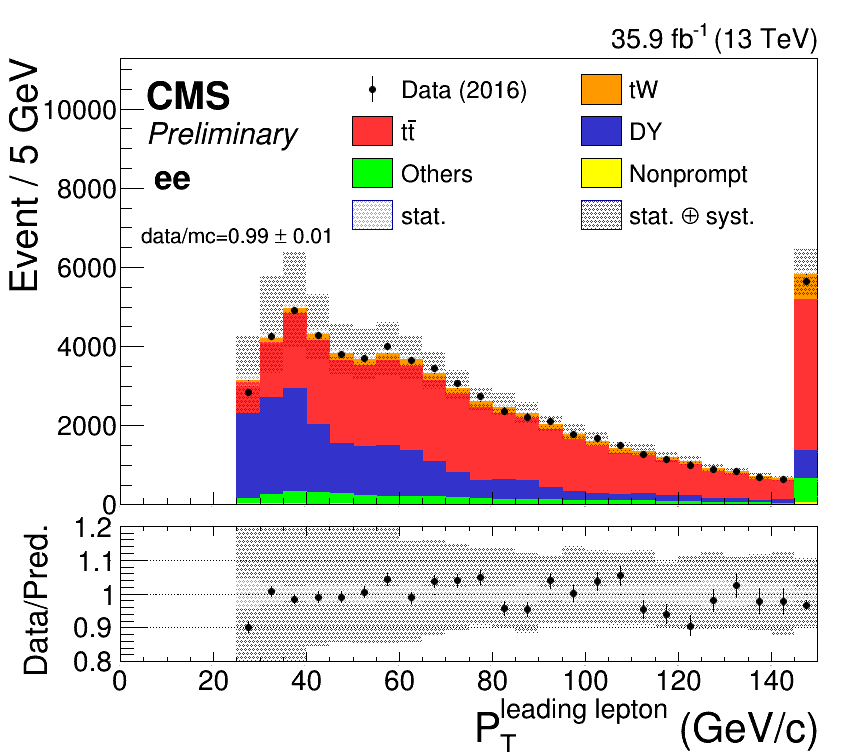
\includegraphics[width=0.4\textwidth]{figures/tW/fig/Step2/ee/H_lepton_led_pt.png}&
      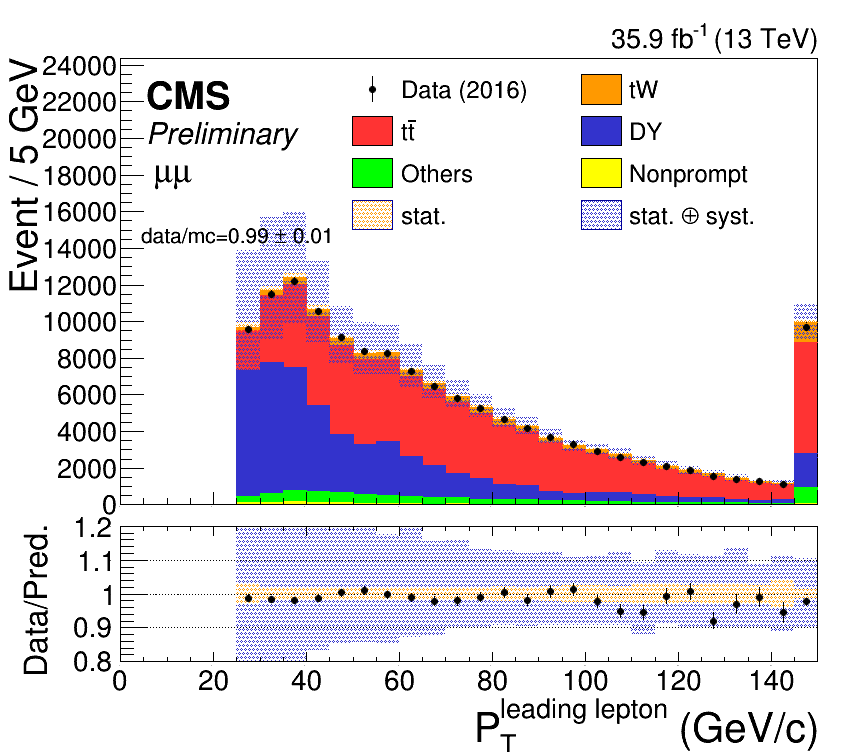
\includegraphics[width=0.4\textwidth]{figures/tW/fig/Step2/mumu/H_lepton_led_pt.png}\\
      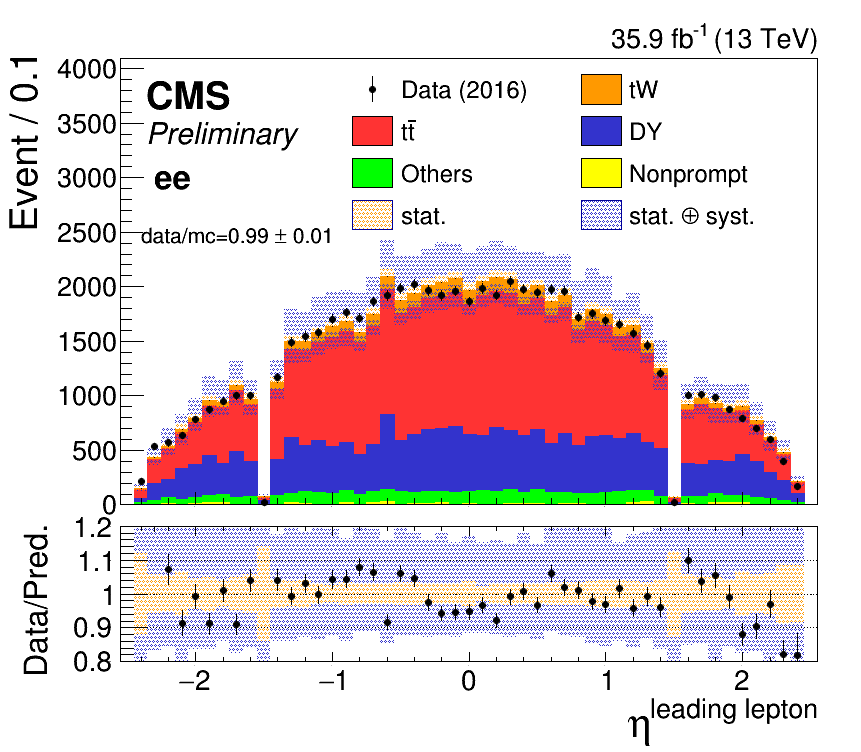
\includegraphics[width=0.4\textwidth]{figures/tW/fig/Step2/ee/H_lepton_led_eta.png}&
      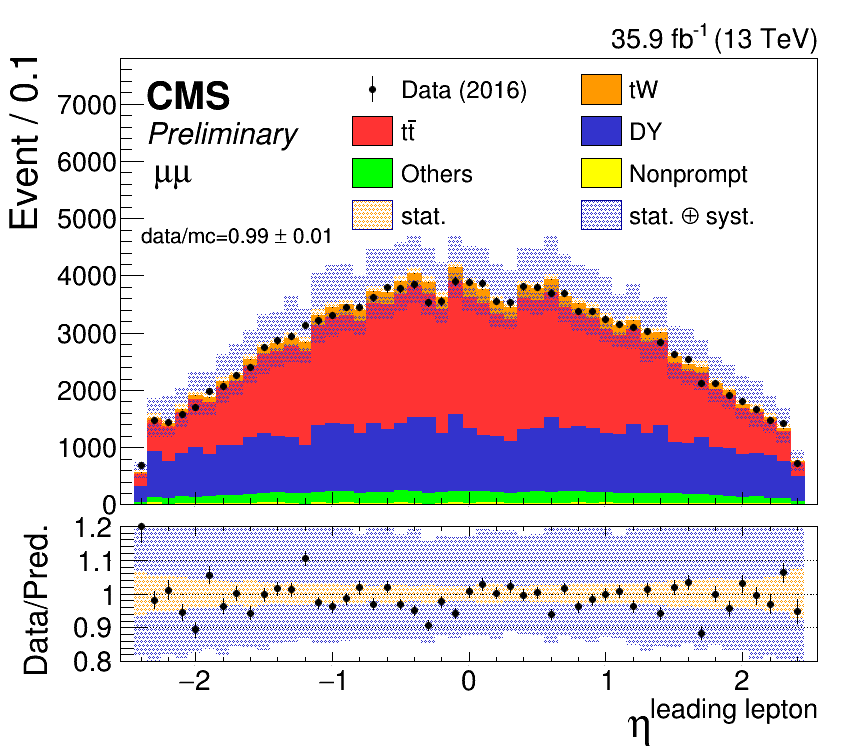
\includegraphics[width=0.4\textwidth]{figures/tW/fig/Step2/mumu/H_lepton_led_eta.png}\\
      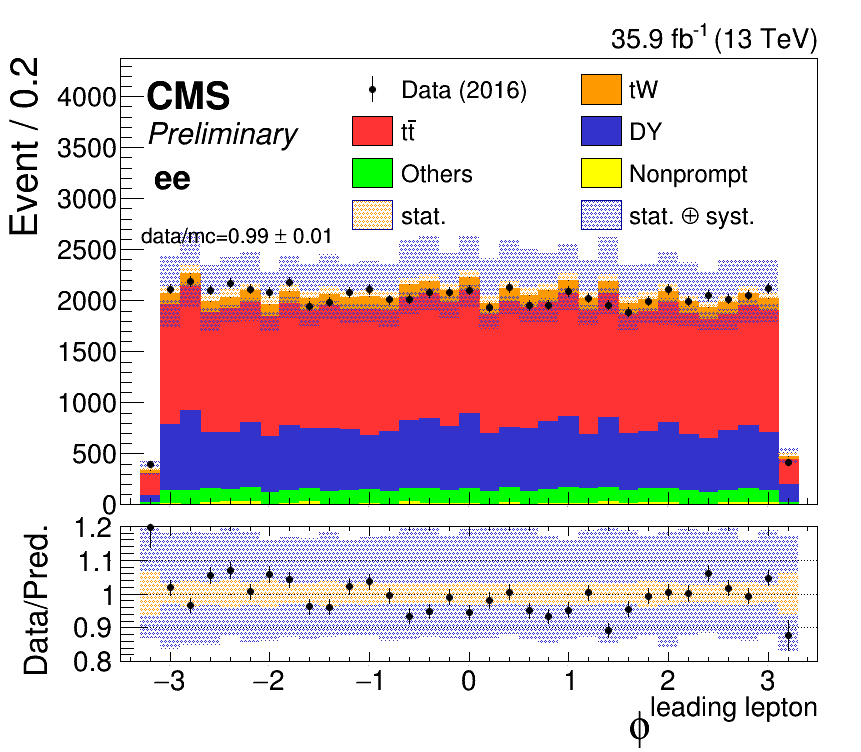
\includegraphics[width=0.4\textwidth]{figures/tW/fig/Step2/ee/H_lepton_led_phi.png}&
      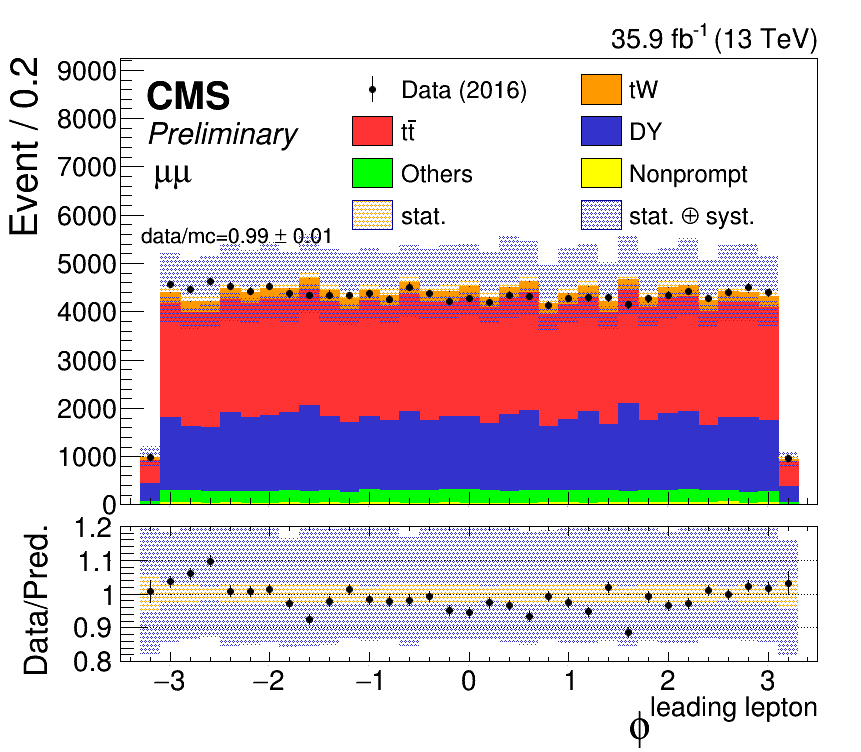
\includegraphics[width=0.4\textwidth]{figures/tW/fig/Step2/mumu/H_lepton_led_phi.png}\\
    \end{tabular}
    \caption{The distributions of \pt (top), $\eta$ (middle) and $\phi$ (bottom) of leading lepton for ee (left) and \mumu (right) channels after step 2 (full selection).
    \label{fig:step2_leading_lepton}}
  \end{center}
\end{figure}

\begin{figure}[ht]
  \begin{center}
    \begin{tabular}{ccc}
      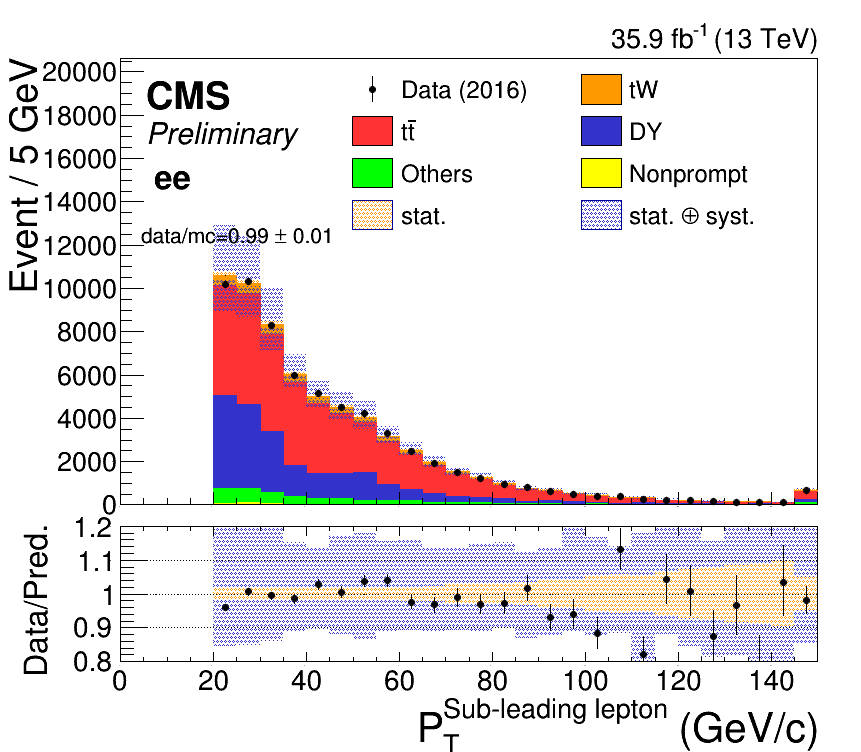
\includegraphics[width=0.4\textwidth]{figures/tW/fig/Step2/ee/H_lepton_sub_pt.png}&
      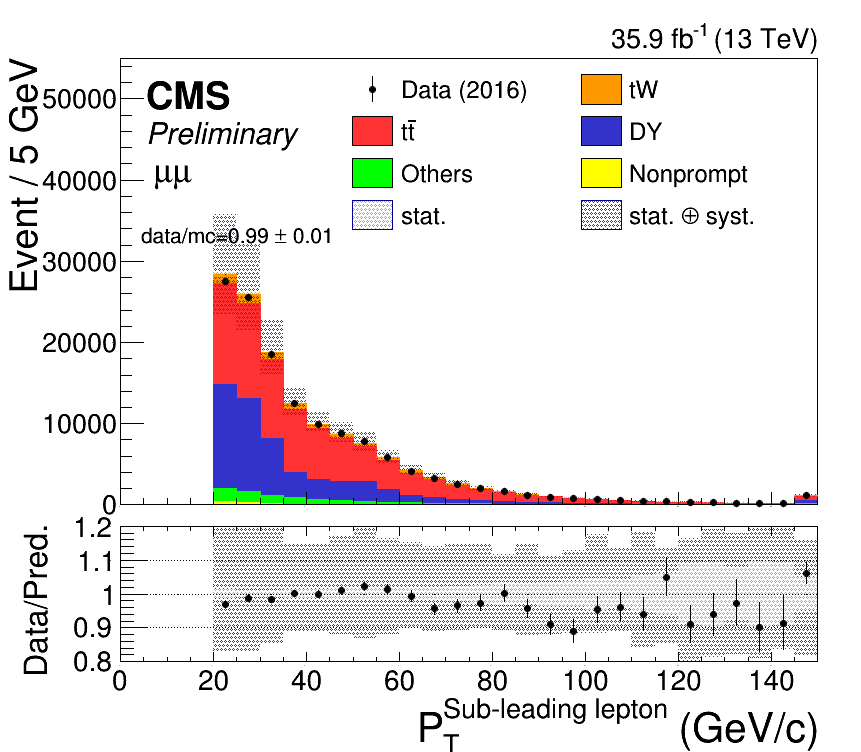
\includegraphics[width=0.4\textwidth]{figures/tW/fig/Step2/mumu/H_lepton_sub_pt.png}\\
      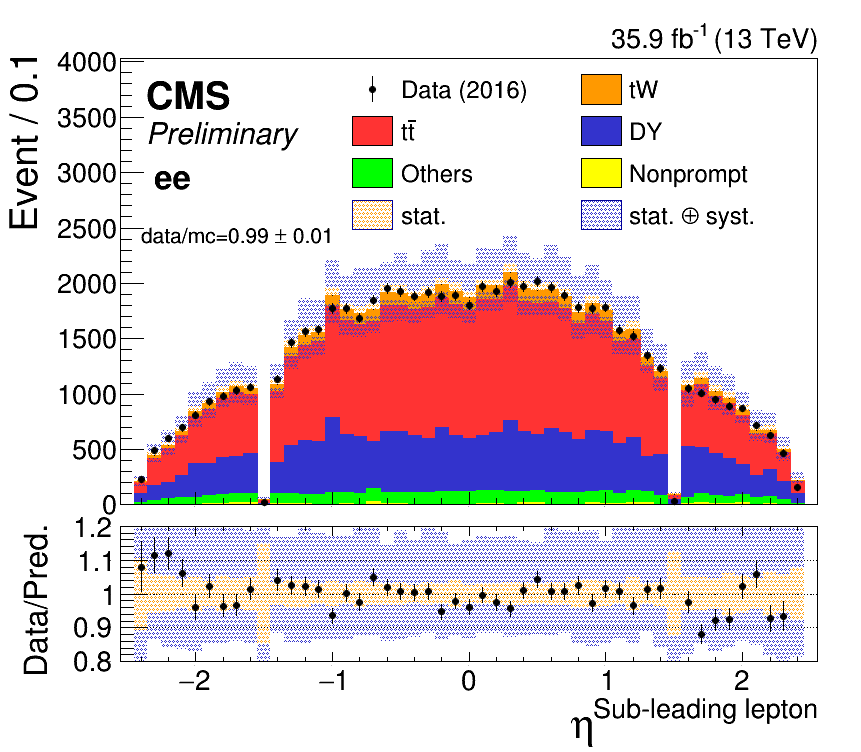
\includegraphics[width=0.4\textwidth]{figures/tW/fig/Step2/ee/H_lepton_sub_eta.png}&
      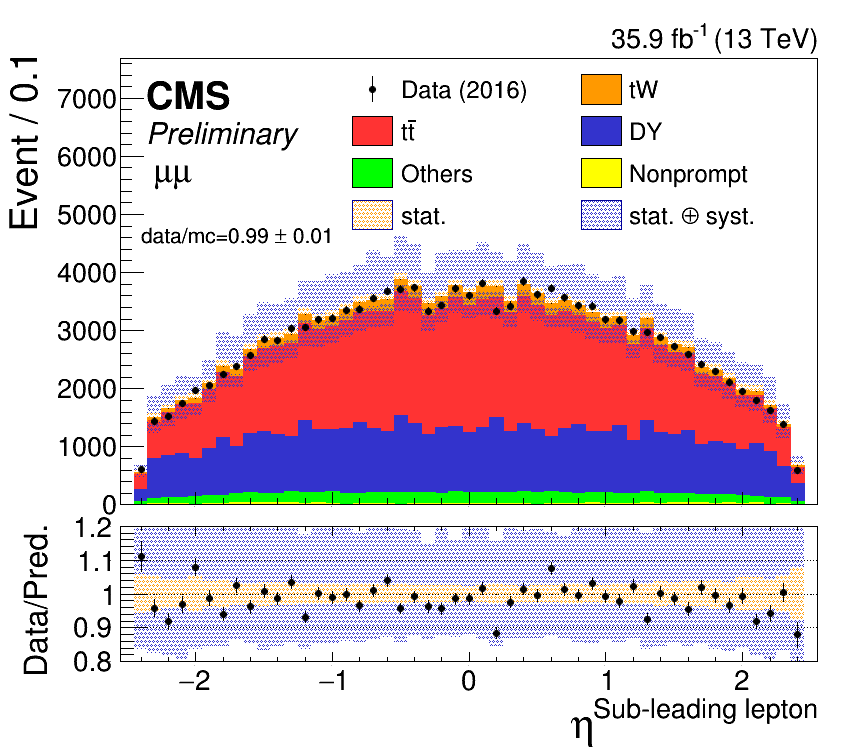
\includegraphics[width=0.4\textwidth]{figures/tW/fig/Step2/mumu/H_lepton_sub_eta.png}\\
      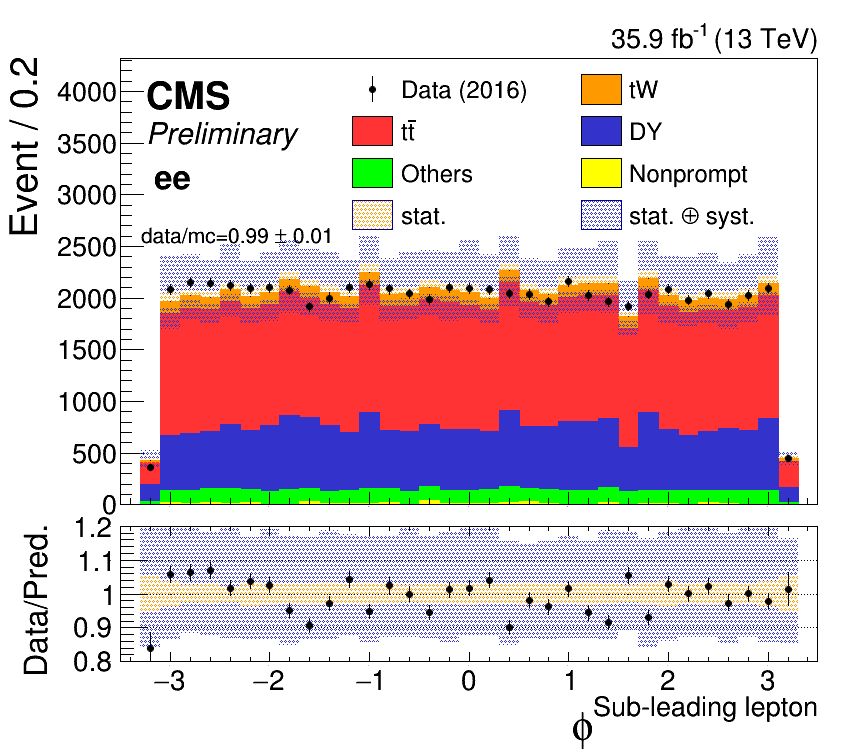
\includegraphics[width=0.4\textwidth]{figures/tW/fig/Step2/ee/H_lepton_sub_phi.png}&
      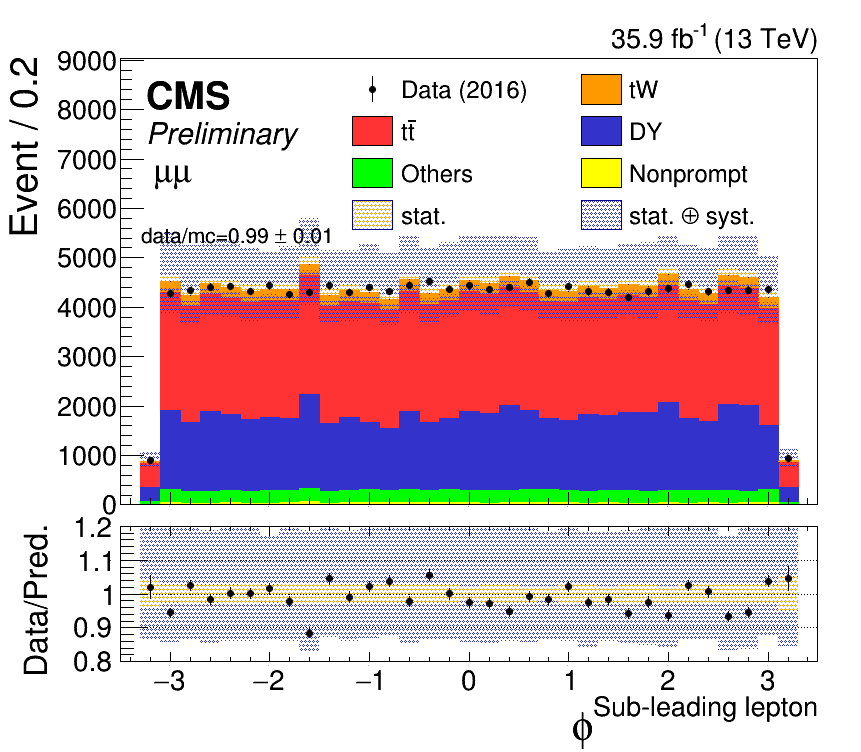
\includegraphics[width=0.4\textwidth]{figures/tW/fig/Step2/mumu/H_lepton_sub_phi.png}\\
    \end{tabular}
    \caption{The distributions of \pt (top), $\eta$ (middle) and $\phi$ (bottom) of sub-leading lepton for ee (left) and \mumu (right) channels after step 2 (full selection).
    \label{fig:step2_subleading_lepton}}
  \end{center}
\end{figure}


\begin{figure}[ht]
  \begin{center}
    \begin{tabular}{ccc}
      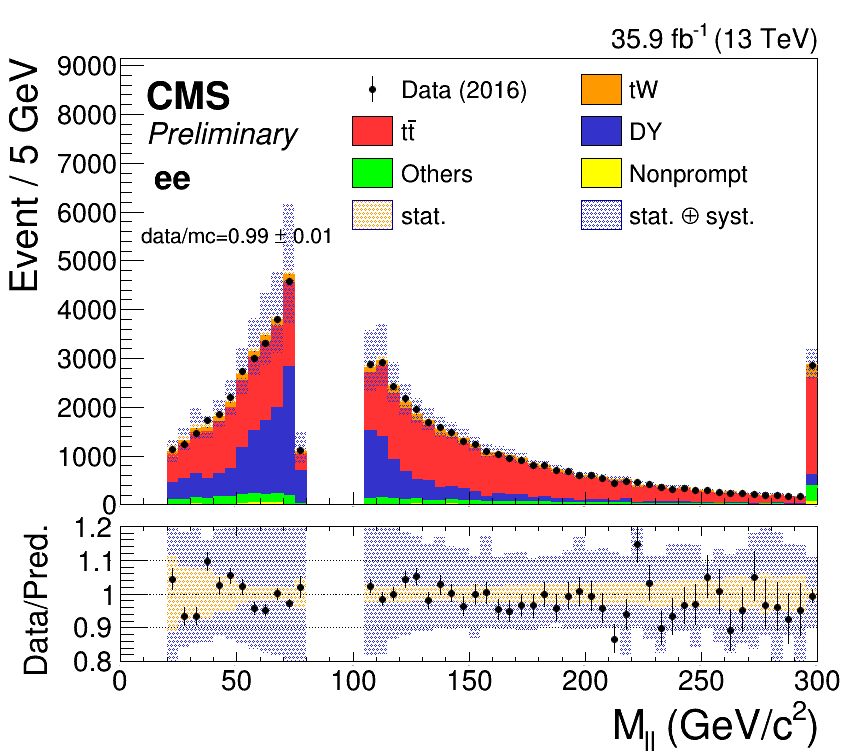
\includegraphics[width=0.4\textwidth]{figures/tW/fig/Step2/ee/H_Mll.png}&
      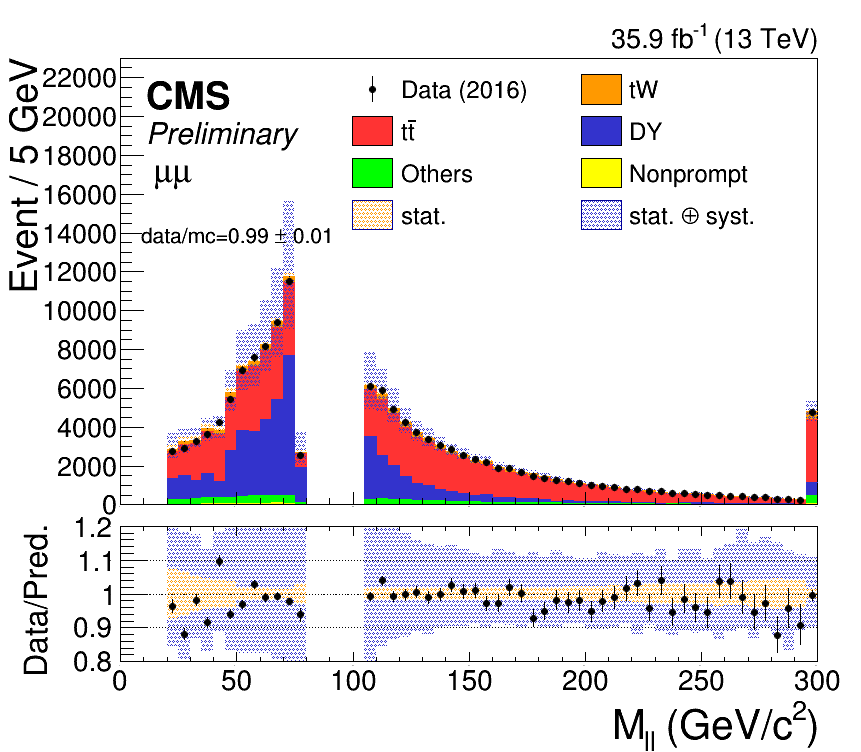
\includegraphics[width=0.4\textwidth]{figures/tW/fig/Step2/mumu/H_Mll.png}\\
      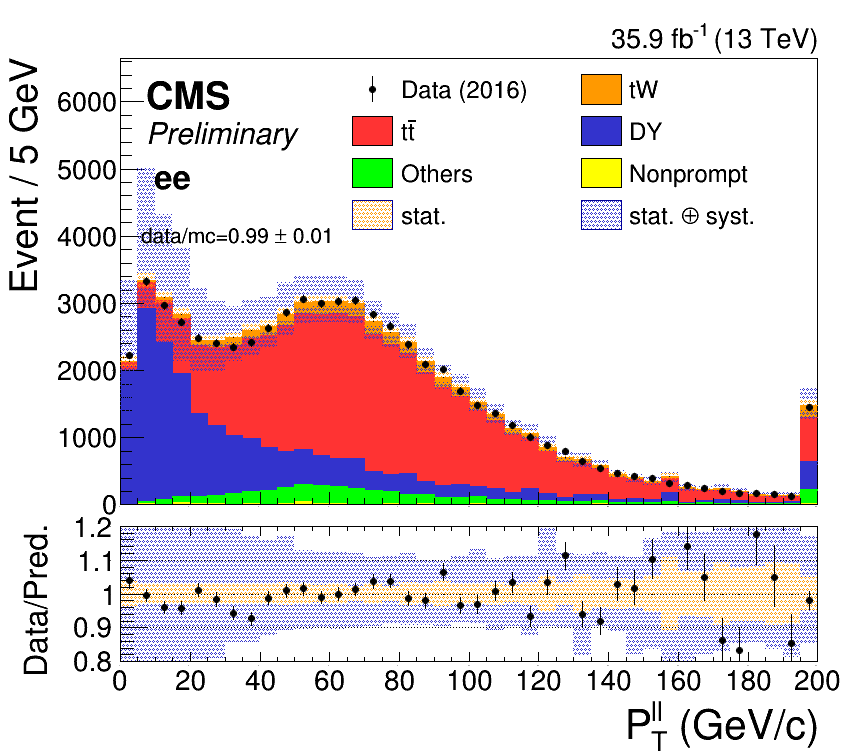
\includegraphics[width=0.4\textwidth]{figures/tW/fig/Step2/ee/H_Ptll.png}&
      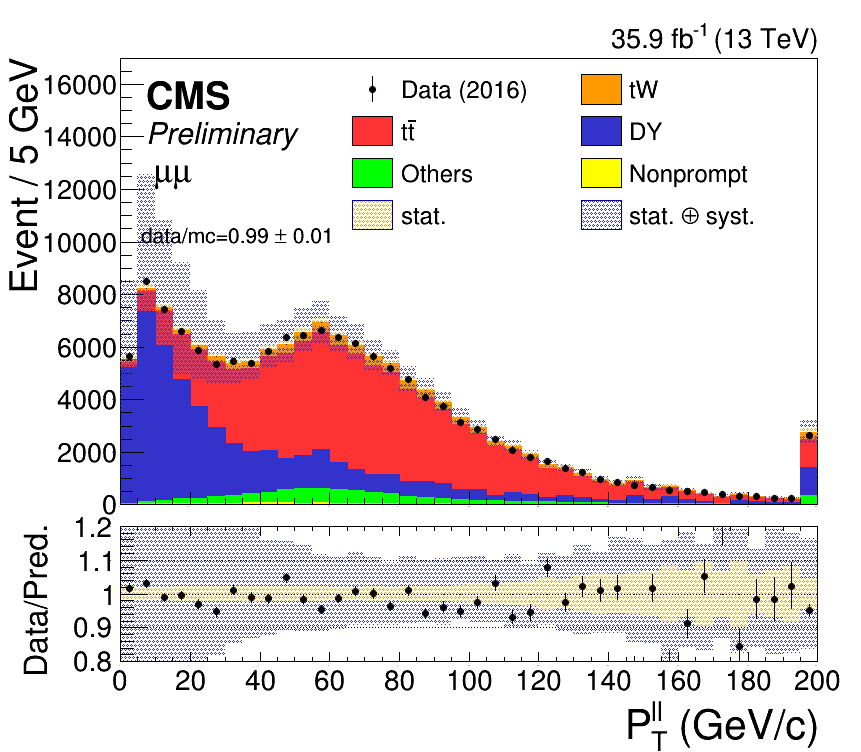
\includegraphics[width=0.4\textwidth]{figures/tW/fig/Step2/mumu/H_Ptll.png}\\
      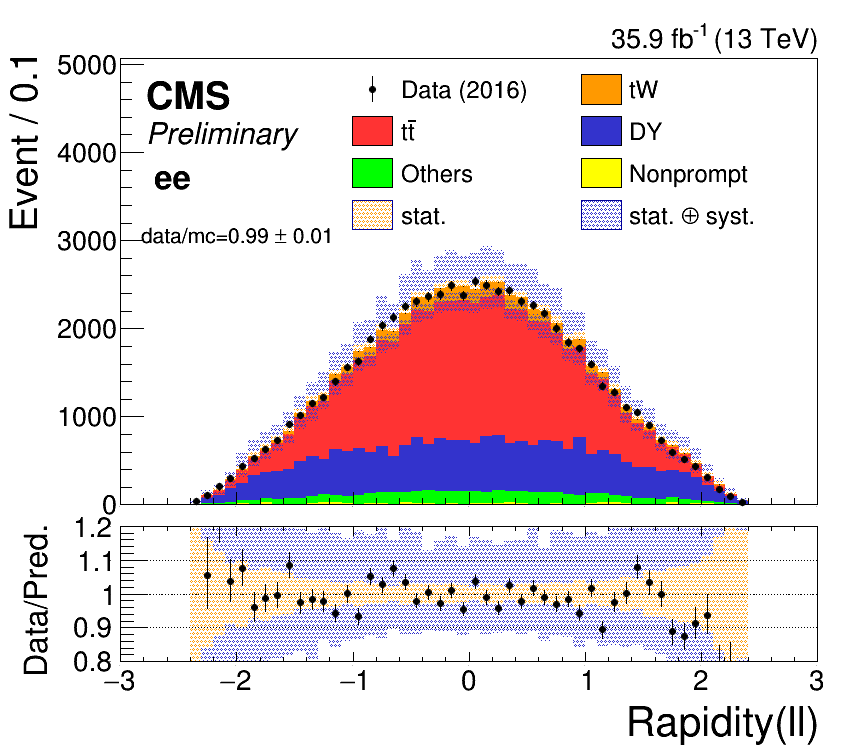
\includegraphics[width=0.4\textwidth]{figures/tW/fig/Step2/ee/H_Rll.png}&
      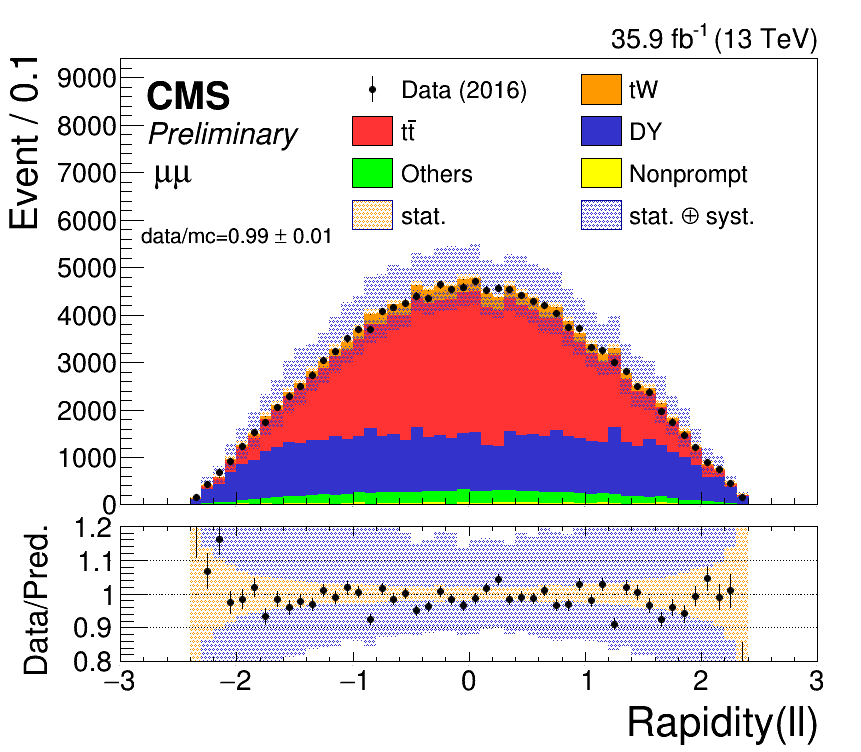
\includegraphics[width=0.4\textwidth]{figures/tW/fig/Step2/mumu/H_Rll.png}\\
      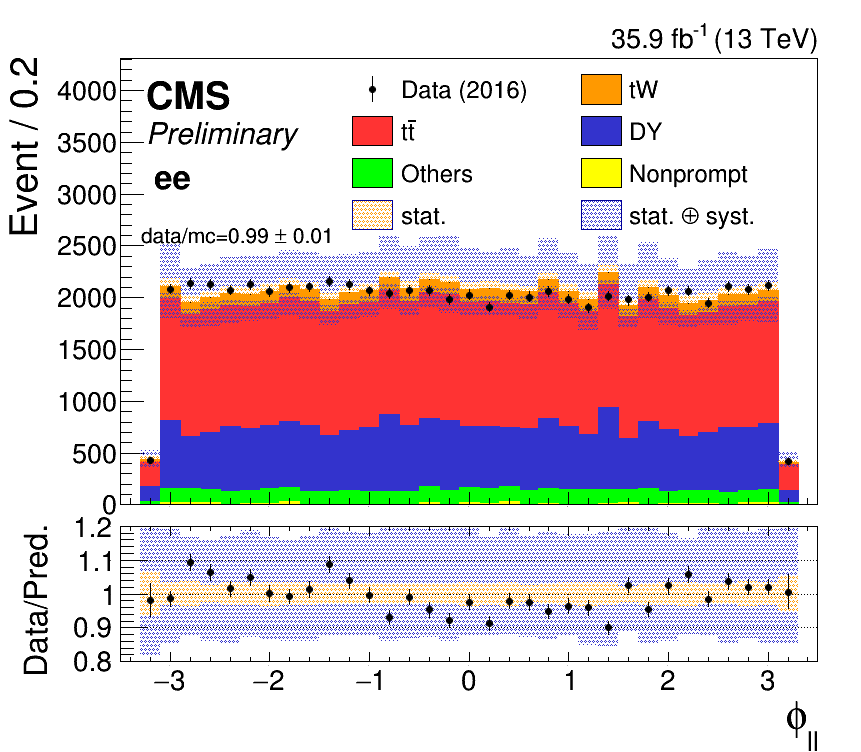
\includegraphics[width=0.4\textwidth]{figures/tW/fig/Step2/ee/H_Ptll_phi.png}&
      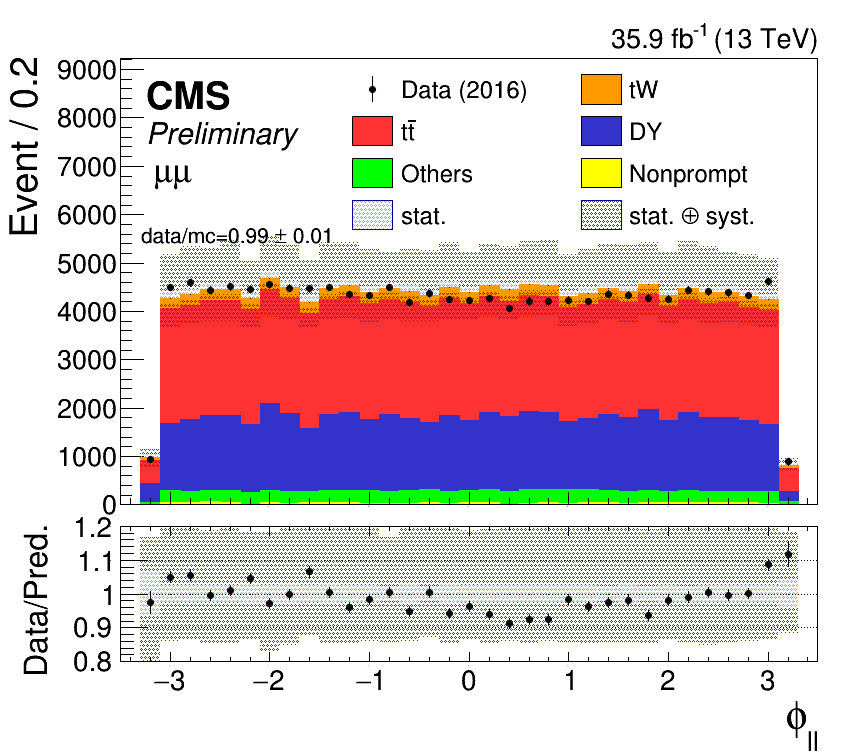
\includegraphics[width=0.4\textwidth]{figures/tW/fig/Step2/mumu/H_Ptll_phi.png}\\
    \end{tabular}
    \caption{The distributions of invariant mass of two leptons (first row), \pt of two leptons (second row), Rapidity of two leptons (third row) and $\phi$ of two leptons (last row) for ee (left) and \mumu (right) channels after step 2 (full selection).
    \label{fig:step2_M_pt_R_phi}}
  \end{center}
\end{figure}


\begin{figure}[ht]
  \begin{center}
    \begin{tabular}{ccc}
      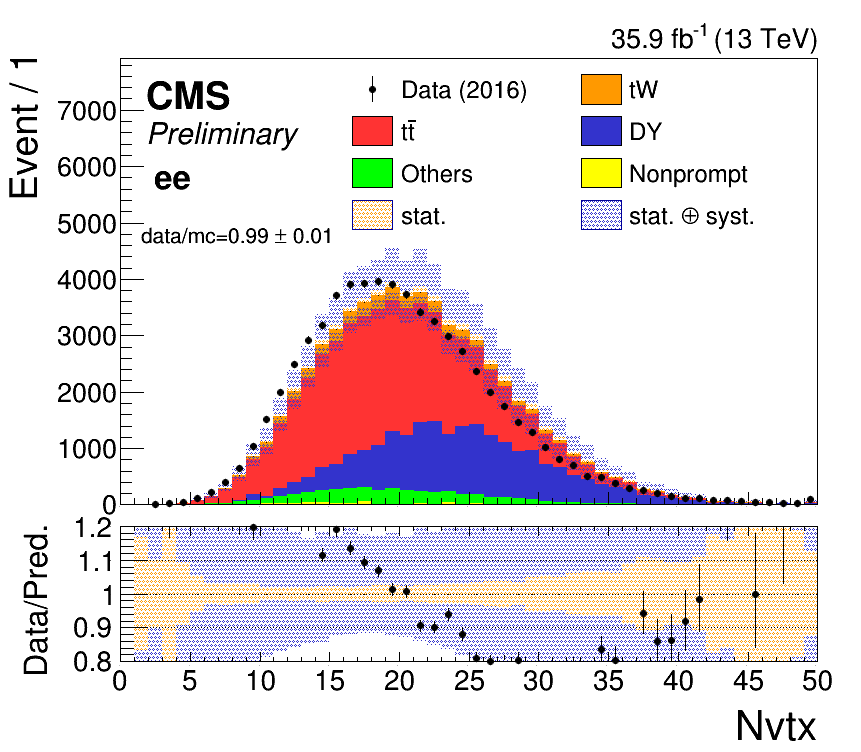
\includegraphics[width=0.4\textwidth]{figures/tW/fig/Step2/ee/H_pv_n.png}&
      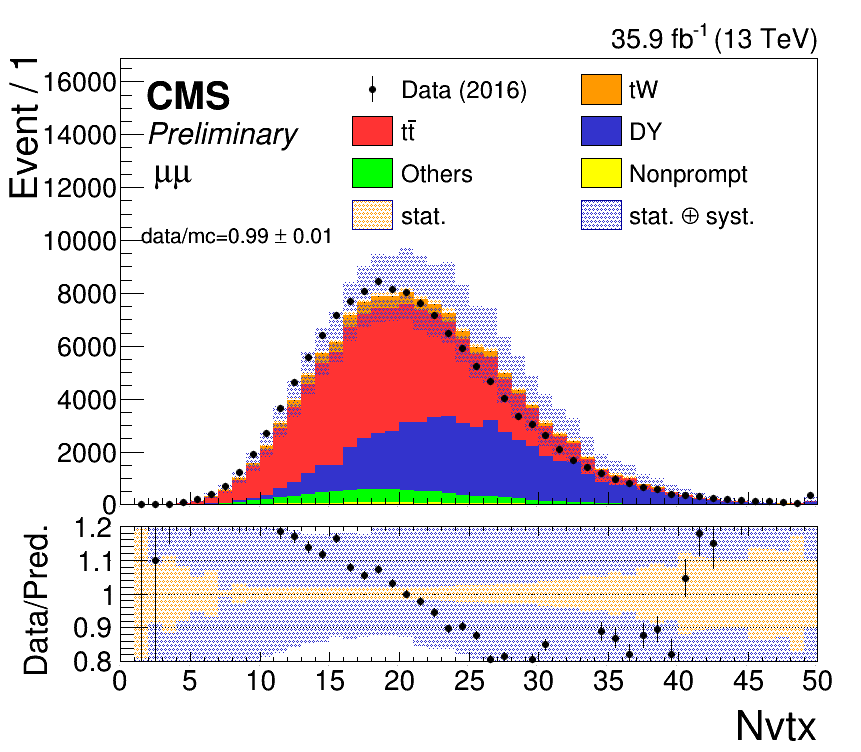
\includegraphics[width=0.4\textwidth]{figures/tW/fig/Step2/mumu/H_pv_n.png}\\
      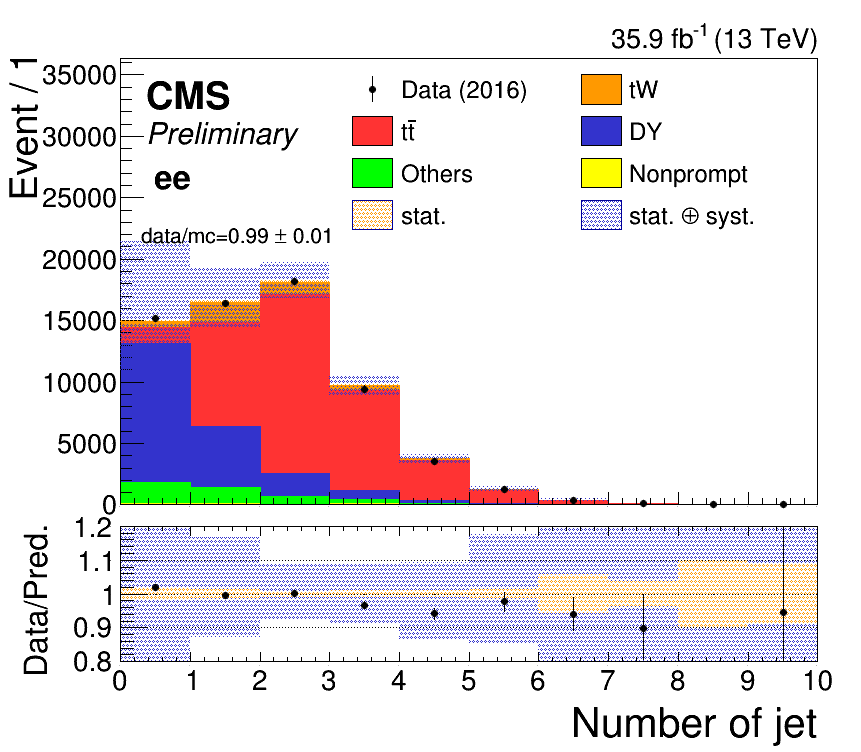
\includegraphics[width=0.4\textwidth]{figures/tW/fig/Step2/ee/H_N_loose_jets.png}&
      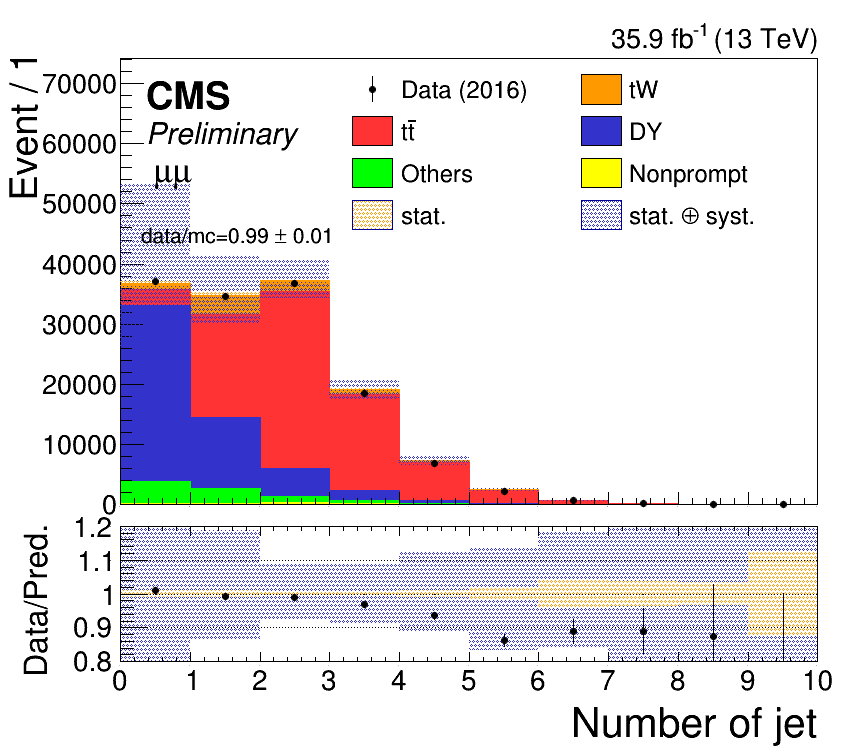
\includegraphics[width=0.4\textwidth]{figures/tW/fig/Step2/mumu/H_N_loose_jets.png}\\
      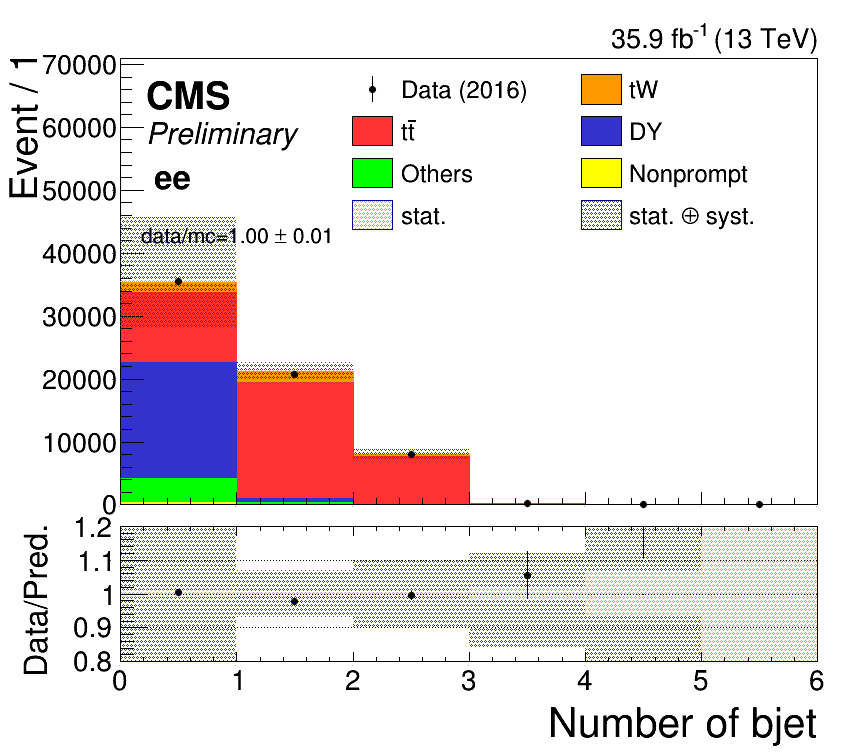
\includegraphics[width=0.4\textwidth]{figures/tW/fig/Step2/ee/H_N_b_jets.png}&
      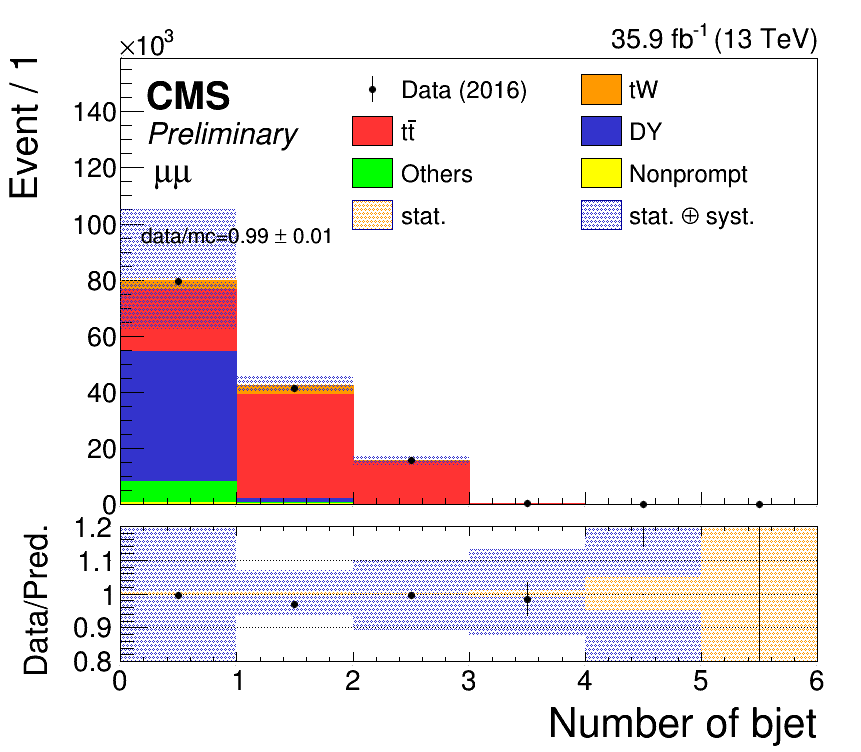
\includegraphics[width=0.4\textwidth]{figures/tW/fig/Step2/mumu/H_N_b_jets.png}\\
      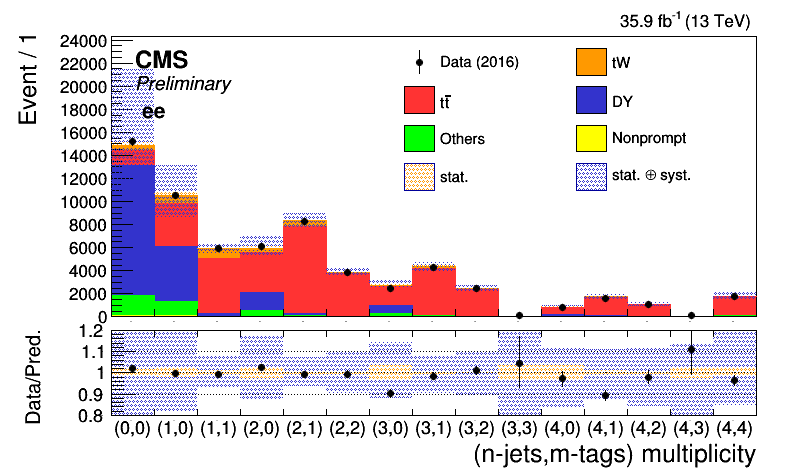
\includegraphics[width=0.4\textwidth]{figures/tW/fig/Step2/ee/H_njet_bjet.png}&
      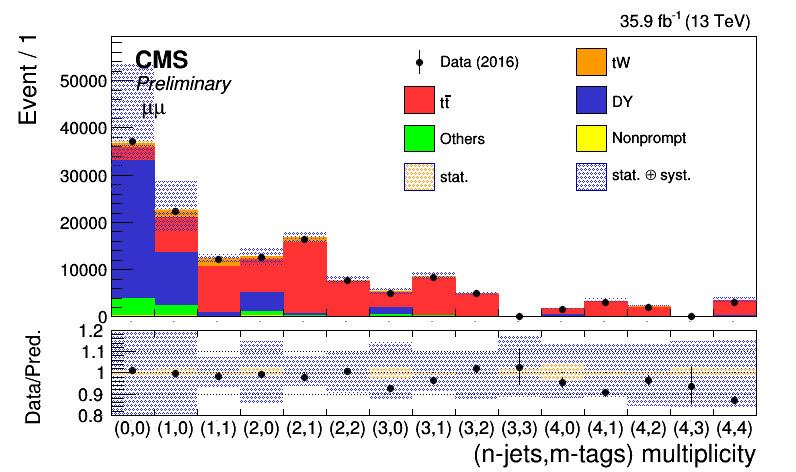
\includegraphics[width=0.4\textwidth]{figures/tW/fig/Step2/mumu/H_njet_bjet.png}\\
    \end{tabular}
    \caption{The distributions of number of vertices (first row), number of jet (second row), number of b jets (third row) and number of jet-bjets (last row) for ee (left) and \mumu (right) channels after step 2 (full selection).
    \label{fig:step2_Nvtx_jet_bjet}}
  \end{center}
\end{figure}


\begin{figure}[ht]
  \begin{center}
    \begin{tabular}{ccc}
      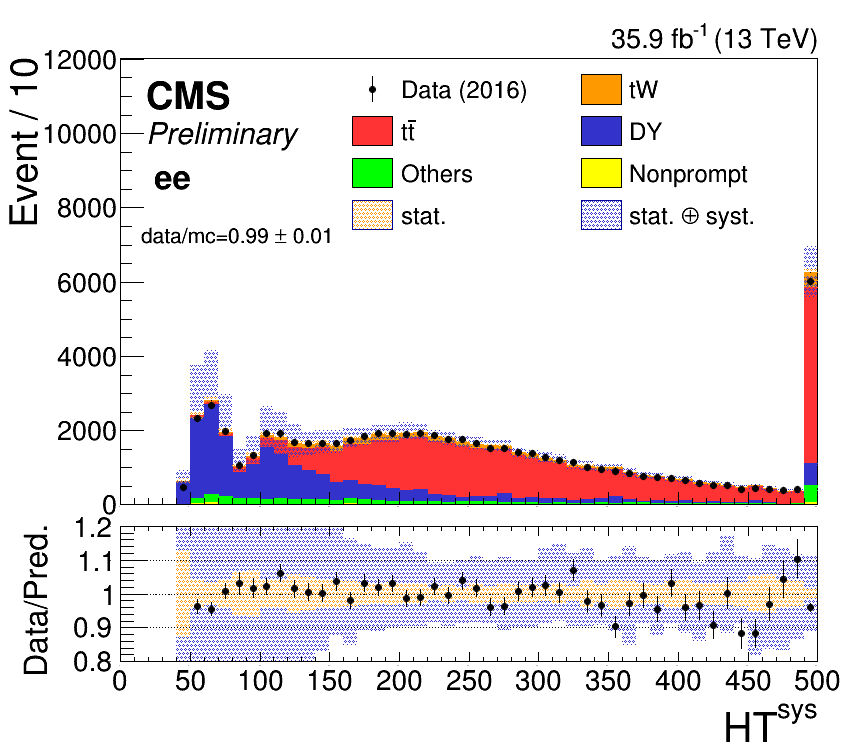
\includegraphics[width=0.4\textwidth]{figures/tW/fig/Step2/ee/H_HT_sys.png}   &
      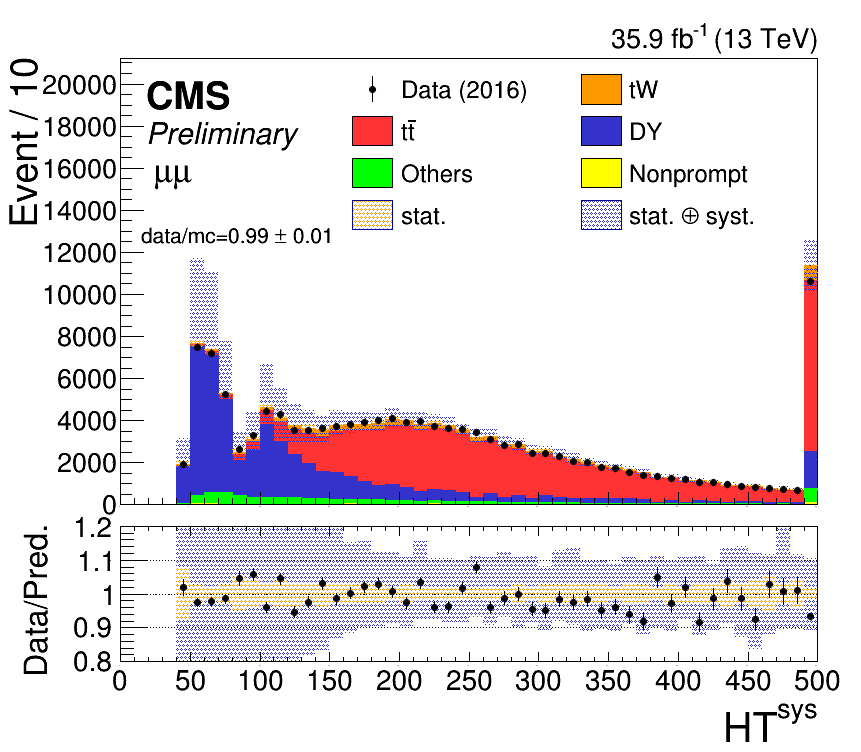
\includegraphics[width=0.4\textwidth]{figures/tW/fig/Step2/mumu/H_HT_sys.png} \\
      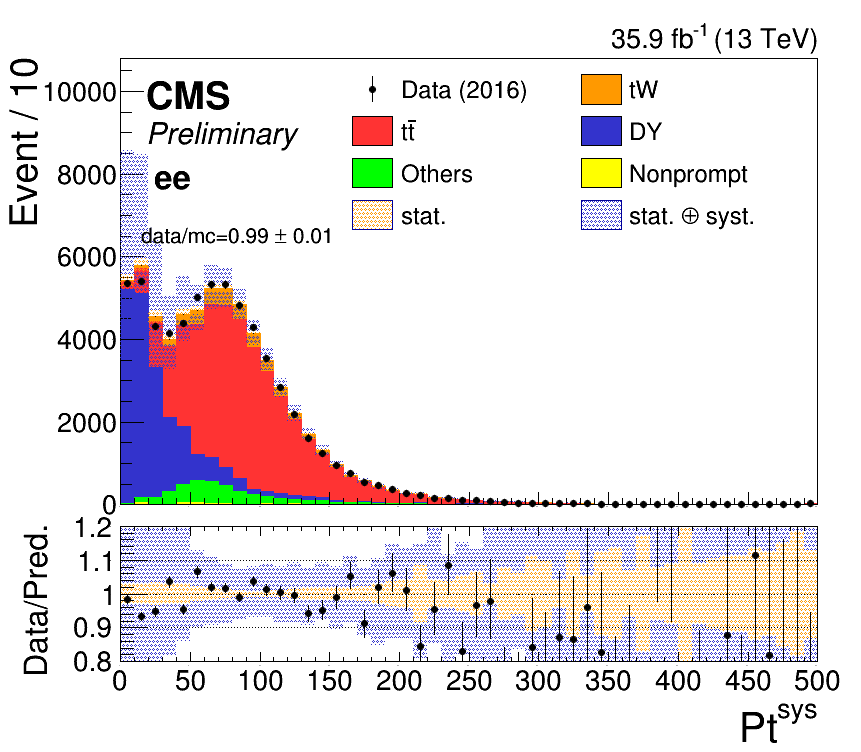
\includegraphics[width=0.4\textwidth]{figures/tW/fig/Step2/ee/H_Pt_sys.png}   &
      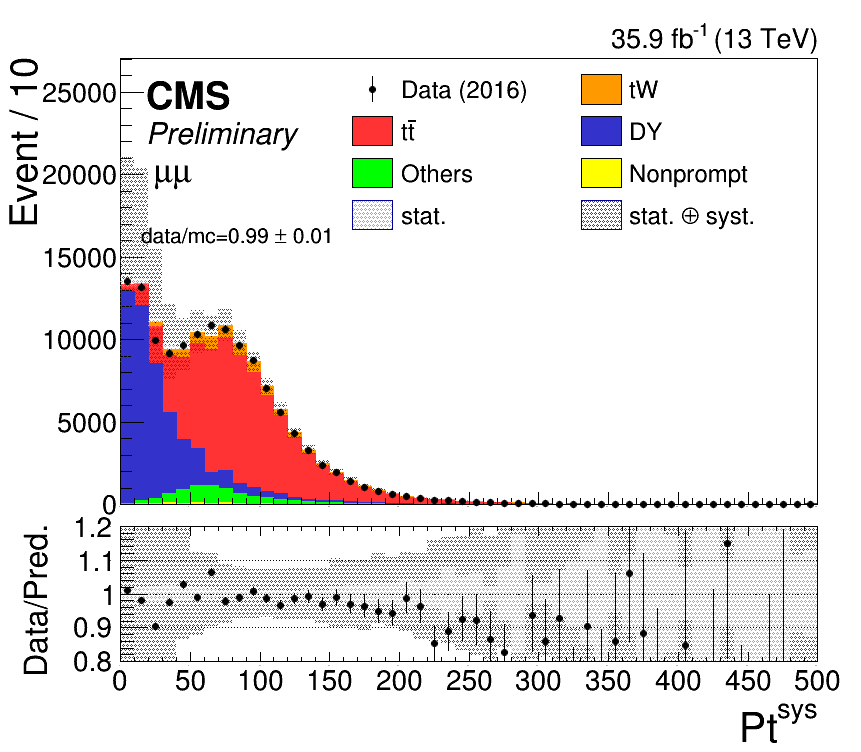
\includegraphics[width=0.4\textwidth]{figures/tW/fig/Step2/mumu/H_Pt_sys.png} \\
      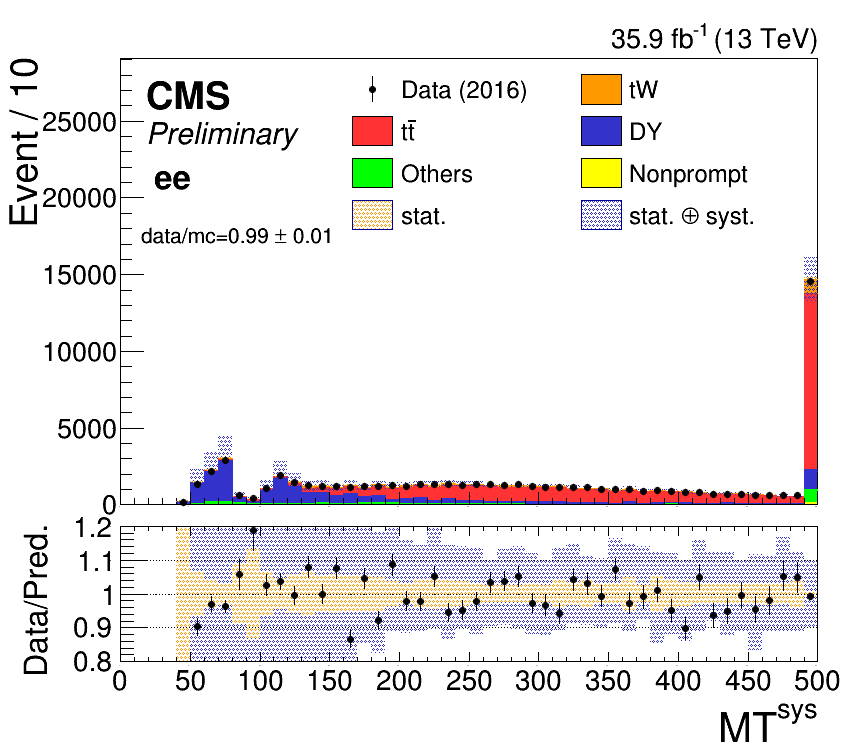
\includegraphics[width=0.4\textwidth]{figures/tW/fig/Step2/ee/H_MT_sys.png}    &
      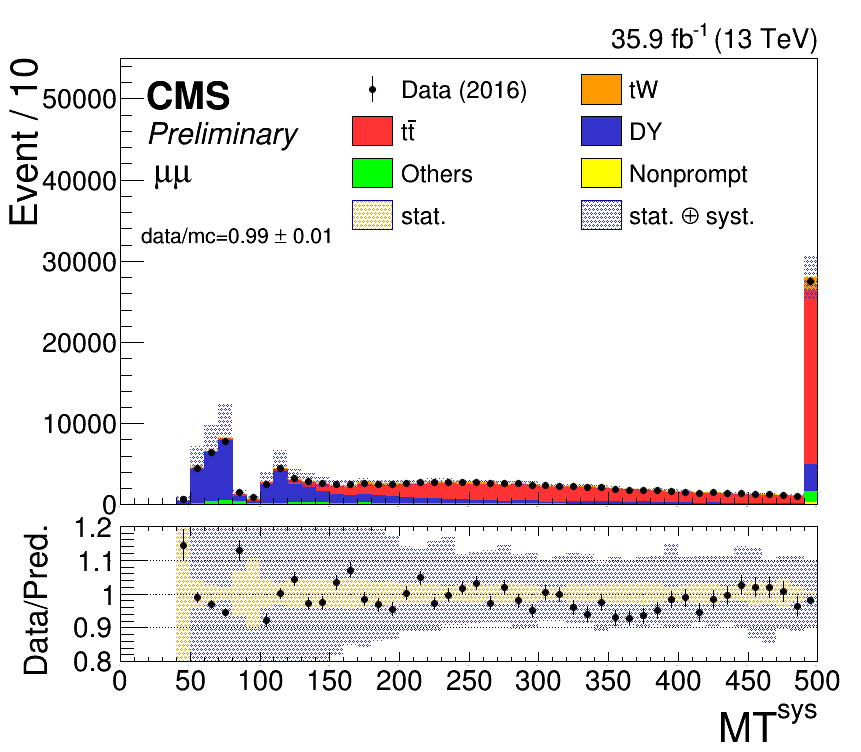
\includegraphics[width=0.4\textwidth]{figures/tW/fig/Step2/mumu/H_MT_sys.png}  \\
      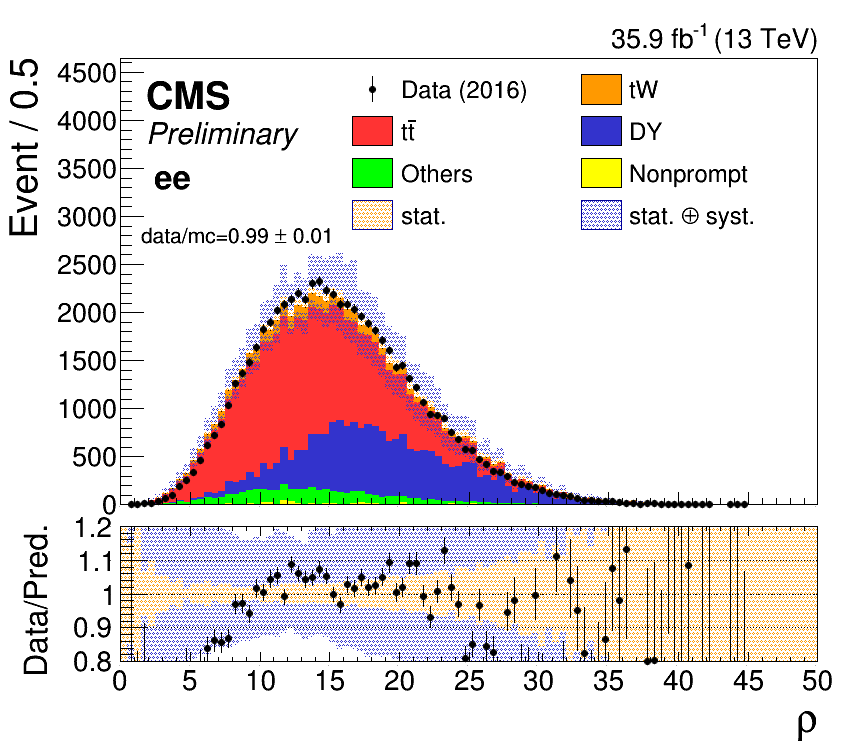
\includegraphics[width=0.4\textwidth]{figures/tW/fig/Step2/ee/H_rho.png}&
      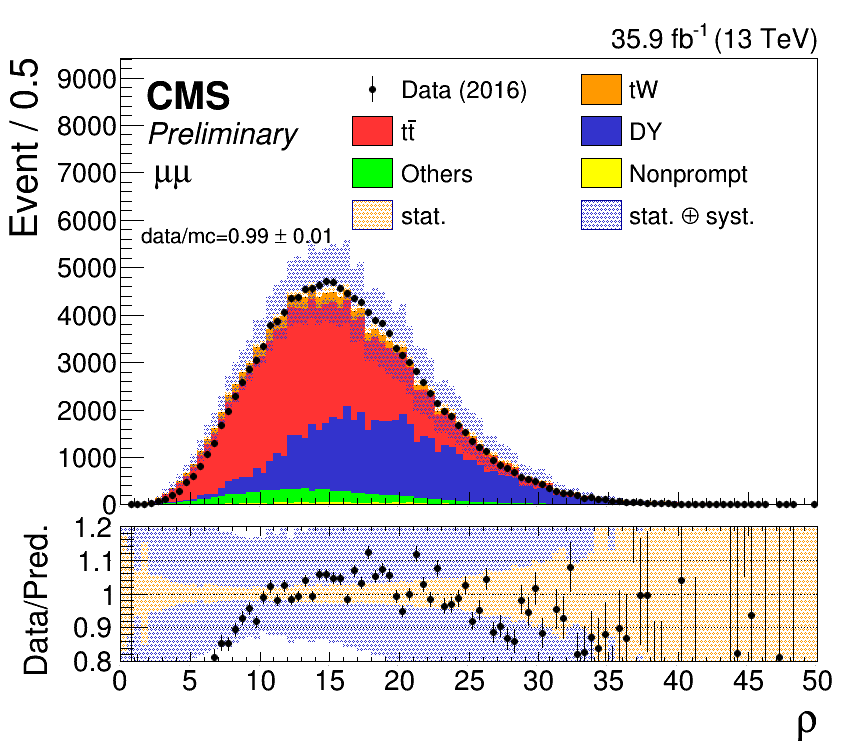
\includegraphics[width=0.4\textwidth]{figures/tW/fig/Step2/mumu/H_rho.png}\\
    \end{tabular}
    \caption{The distributions of $\mathrm{HT^{syst}}$ (first row), $\mathrm{\pt^{syst}}$ (second row), $\mathrm{MT^{syst}}$ (third row)  and $\rho$ for ee (left) and \mumu (right) channels after step 2 (full selection).
    \label{fig:step2_HT_Pt_Mt_rho}}
  \end{center}
\end{figure}




\begin{figure}[ht]
  \begin{center}
    \begin{tabular}{ccc}
      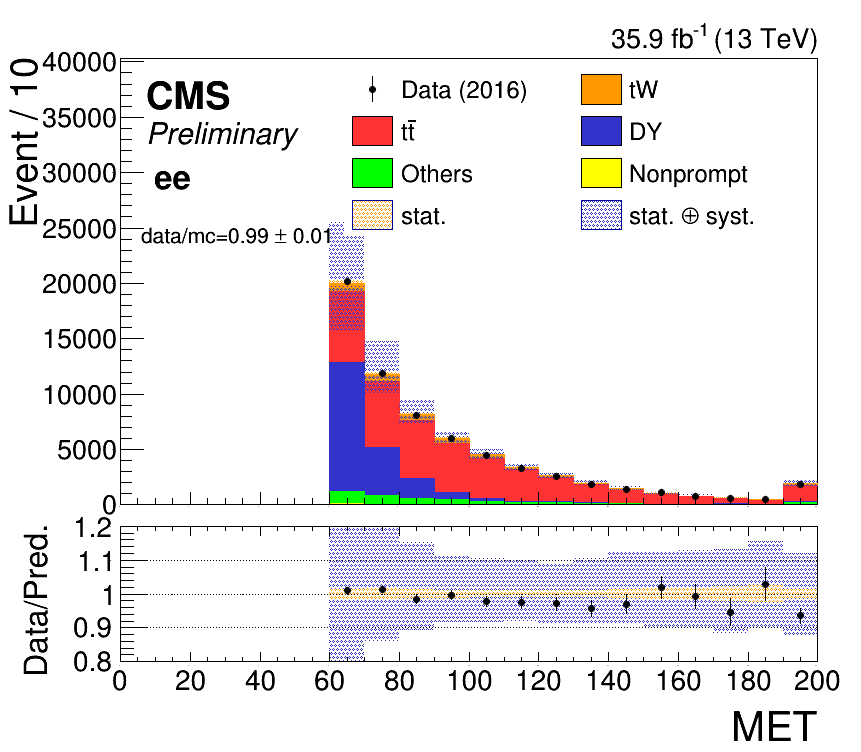
\includegraphics[width=0.4\textwidth]{figures/tW/fig/Step2/ee/H_MET_Et.png}&
      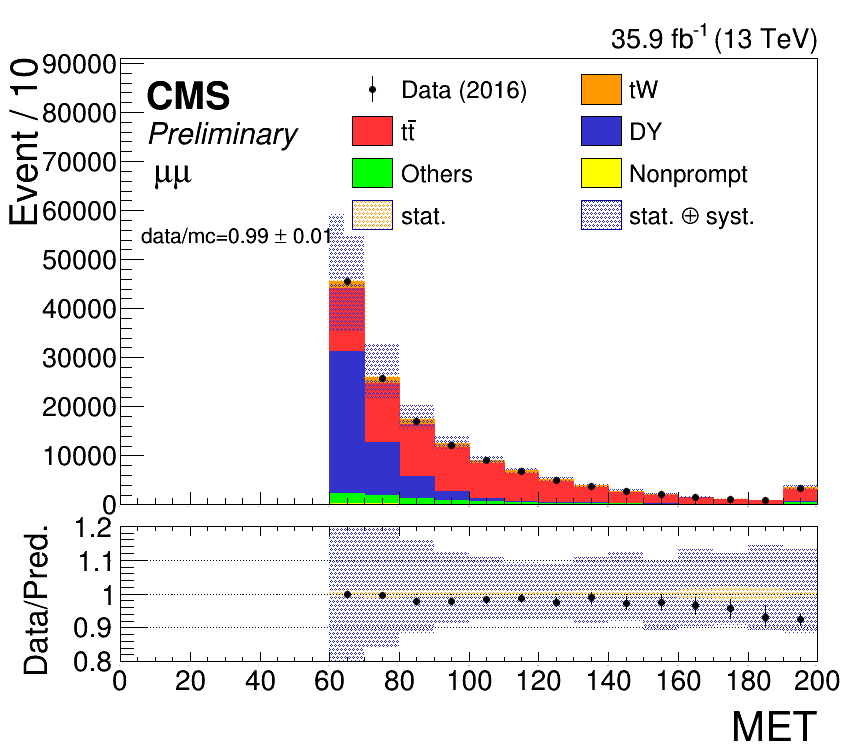
\includegraphics[width=0.4\textwidth]{figures/tW/fig/Step2/mumu/H_MET_Et.png}\\
%      \includegraphics[width=0.4\textwidth]{figures/tW/fig/Step2/ee/H_MET_phi.png}&
%      \includegraphics[width=0.4\textwidth]{figures/tW/fig/Step2/mumu/H_MET_phi.png}\\
      \includegraphics[width=0.4\textwidth]{figures/tW/fig/Step2/ee/H_ll_Dphi.png}&
      \includegraphics[width=0.4\textwidth]{figures/tW/fig/Step2/mumu/H_ll_Dphi.png}\\
      \includegraphics[width=0.4\textwidth]{figures/tW/fig/Step2/ee/H_ll_DR.png}&
      \includegraphics[width=0.4\textwidth]{figures/tW/fig/Step2/mumu/H_ll_DR.png}\\
    \end{tabular}
    \caption{The distributions of MET (top row), $\Delta\phi$ between two leptons (middle row) and $\Delta R$ between two leptons (bottom row) for ee (left) and \mumu (right) channels after step 2 (full selection).
    \label{fig:step2_MET_phi_Dphi_DR}}
  \end{center}
\end{figure}

\begin{figure}[ht]
  \begin{center}
    \begin{tabular}{cc}
      \includegraphics[width=0.45\textwidth]{figures/tW/fig/Result/ee/H_Limit_N_jet_bjet.png}&
      \includegraphics[width=0.45\textwidth]{figures/tW/fig/Result/mumu/H_Limit_N_jet_bjet.png}\\
    \end{tabular}
    \caption{The observed numbers of events and SM background predictions in the search regions of the analysis for the ee (left), \mumu (right) channels. The hatched band corresponds to the quadratic sum of statistical and systematic uncertainties in the event yield for the SM background predictions. The ratios of data to the sum of the predicted yields are shown at the bottom of each plot. The narrow hatched band represents the contribution from the statistical uncertainty in the MC simulation.
    \label{fig:binee}}
  \end{center}
\end{figure}



\clearpage







%\begin{figure}[ht]
%  \begin{center}
%    \begin{tabular}{ccc}
%      \includegraphics[width=0.32\textwidth]{figures/tW/fig/Step2/ee/H_lepton_led_pt.png}&
%      \includegraphics[width=0.32\textwidth]{figures/tW/fig/Step2/emu/H_lepton_led_pt.png}&
%      \includegraphics[width=0.32\textwidth]{figures/tW/fig/Step2/mumu/H_lepton_led_pt.png}\\
%      \includegraphics[width=0.32\textwidth]{figures/tW/fig/Step2/ee/H_lepton_led_eta.png}&
%      \includegraphics[width=0.32\textwidth]{figures/tW/fig/Step2/emu/H_lepton_led_eta.png}&
%      \includegraphics[width=0.32\textwidth]{figures/tW/fig/Step2/mumu/H_lepton_led_eta.png}\\
%      \includegraphics[width=0.32\textwidth]{figures/tW/fig/Step2/ee/H_lepton_led_phi.png}&
%      \includegraphics[width=0.32\textwidth]{figures/tW/fig/Step2/emu/H_lepton_led_phi.png}&
%      \includegraphics[width=0.32\textwidth]{figures/tW/fig/Step2/mumu/H_lepton_led_phi.png}\\
%    \end{tabular}
%    \caption{The distributions of Pt (top), $\eta$ (middle) and $\phi$ (bottom) of leading lepton for ee (left), $e\mu$ (middle) and \mumu (right) channels after step 2 (full selection).
%    \label{fig:step2_leading_lepton}}
%  \end{center}
%\end{figure}
%
%\begin{figure}[ht]
%  \begin{center}
%    \begin{tabular}{ccc}
%      \includegraphics[width=0.32\textwidth]{figures/tW/fig/Step2/ee/H_lepton_sub_pt.png}&
%      \includegraphics[width=0.32\textwidth]{figures/tW/fig/Step2/emu/H_lepton_sub_pt.png}&
%      \includegraphics[width=0.32\textwidth]{figures/tW/fig/Step2/mumu/H_lepton_sub_pt.png}\\
%      \includegraphics[width=0.32\textwidth]{figures/tW/fig/Step2/ee/H_lepton_sub_eta.png}&
%      \includegraphics[width=0.32\textwidth]{figures/tW/fig/Step2/emu/H_lepton_sub_eta.png}&
%      \includegraphics[width=0.32\textwidth]{figures/tW/fig/Step2/mumu/H_lepton_sub_eta.png}\\
%      \includegraphics[width=0.32\textwidth]{figures/tW/fig/Step2/ee/H_lepton_sub_phi.png}&
%      \includegraphics[width=0.32\textwidth]{figures/tW/fig/Step2/emu/H_lepton_sub_phi.png}&
%      \includegraphics[width=0.32\textwidth]{figures/tW/fig/Step2/mumu/H_lepton_sub_phi.png}\\
%    \end{tabular}
%    \caption{The distributions of Pt (top), $\eta$ (middle) and $\phi$ (bottom) of sub-leading lepton for ee (left), $e\mu$ (middle) and \mumu (right) channels after step 2 (full selection).
%    \label{fig:step2_subleading_lepton}}
%  \end{center}
%\end{figure}
%
%
%\begin{figure}[ht]
%  \begin{center}
%    \begin{tabular}{ccc}
%      \includegraphics[width=0.32\textwidth]{figures/tW/fig/Step2/ee/H_Mll.png}&
%      \includegraphics[width=0.32\textwidth]{figures/tW/fig/Step2/emu/H_Mll.png}&
%      \includegraphics[width=0.32\textwidth]{figures/tW/fig/Step2/mumu/H_Mll.png}\\
%      \includegraphics[width=0.32\textwidth]{figures/tW/fig/Step2/ee/H_Ptll.png}&
%      \includegraphics[width=0.32\textwidth]{figures/tW/fig/Step2/emu/H_Ptll.png}&
%      \includegraphics[width=0.32\textwidth]{figures/tW/fig/Step2/mumu/H_Ptll.png}\\
%      \includegraphics[width=0.32\textwidth]{figures/tW/fig/Step2/ee/H_Rll.png}&
%      \includegraphics[width=0.32\textwidth]{figures/tW/fig/Step2/emu/H_Rll.png}&
%      \includegraphics[width=0.32\textwidth]{figures/tW/fig/Step2/mumu/H_Rll.png}\\
%      \includegraphics[width=0.32\textwidth]{figures/tW/fig/Step2/ee/H_Ptll_phi.png}&
%      \includegraphics[width=0.32\textwidth]{figures/tW/fig/Step2/emu/H_Ptll_phi.png}&
%      \includegraphics[width=0.32\textwidth]{figures/tW/fig/Step2/mumu/H_Ptll_phi.png}\\
%    \end{tabular}
%    \caption{The distributions of invariant mass of two leptons (first row), Pt of two leptons (second row), Rapidity of two leptons (third row) and $\phi$ of two leptons (last row) for ee (left), $e\mu$ (middle) and \mumu (right) channels after step 2 (full selection).
%    \label{fig:step2_M_pt_R_phi}}
%  \end{center}
%\end{figure}
%
%
%\begin{figure}[ht]
%  \begin{center}
%    \begin{tabular}{ccc}
%      \includegraphics[width=0.32\textwidth]{figures/tW/fig/Step2/ee/H_pv_n.png}&
%      \includegraphics[width=0.32\textwidth]{figures/tW/fig/Step2/emu/H_pv_n.png}&
%      \includegraphics[width=0.32\textwidth]{figures/tW/fig/Step2/mumu/H_pv_n.png}\\
%      \includegraphics[width=0.32\textwidth]{figures/tW/fig/Step2/ee/H_N_loose_jets.png}&
%      \includegraphics[width=0.32\textwidth]{figures/tW/fig/Step2/emu/H_N_loose_jets.png}&
%      \includegraphics[width=0.32\textwidth]{figures/tW/fig/Step2/mumu/H_N_loose_jets.png}\\
%      \includegraphics[width=0.32\textwidth]{figures/tW/fig/Step2/ee/H_N_b_jets.png}&
%      \includegraphics[width=0.32\textwidth]{figures/tW/fig/Step2/emu/H_N_b_jets.png}&
%      \includegraphics[width=0.32\textwidth]{figures/tW/fig/Step2/mumu/H_N_b_jets.png}\\
%      \includegraphics[width=0.32\textwidth]{figures/tW/fig/Step2/ee/H_njet_bjet.png}&
%      \includegraphics[width=0.32\textwidth]{figures/tW/fig/Step2/emu/H_njet_bjet.png}&
%      \includegraphics[width=0.32\textwidth]{figures/tW/fig/Step2/mumu/H_njet_bjet.png}\\
%    \end{tabular}
%    \caption{The distributions of number of vertices (first row), number of jet (second row), number of b jet (third row) and number of jet-bjet (last row) for ee (left), $e\mu$ (middle) and \mumu (right) channels after step 2 (full selection).
%    \label{fig:step2_Nvtx_jet_bjet}}
%  \end{center}
%\end{figure}
%
%
%\begin{figure}[ht]
%  \begin{center}
%    \begin{tabular}{ccc}
%      \includegraphics[width=0.32\textwidth]{figures/tW/fig/Step2/ee/H_HT_sys.png}   &
%      \includegraphics[width=0.32\textwidth]{figures/tW/fig/Step2/emu/H_HT_sys.png}  &
%      \includegraphics[width=0.32\textwidth]{figures/tW/fig/Step2/mumu/H_HT_sys.png} \\
%      \includegraphics[width=0.32\textwidth]{figures/tW/fig/Step2/ee/H_Pt_sys.png}   &
%      \includegraphics[width=0.32\textwidth]{figures/tW/fig/Step2/emu/H_Pt_sys.png}  &
%      \includegraphics[width=0.32\textwidth]{figures/tW/fig/Step2/mumu/H_Pt_sys.png} \\
%      \includegraphics[width=0.32\textwidth]{figures/tW/fig/Step2/ee/H_MT_sys.png}    &
%      \includegraphics[width=0.32\textwidth]{figures/tW/fig/Step2/emu/H_MT_sys.png}   &
%      \includegraphics[width=0.32\textwidth]{figures/tW/fig/Step2/mumu/H_MT_sys.png}  \\
%      \includegraphics[width=0.32\textwidth]{figures/tW/fig/Step2/ee/H_rho.png}&
%      \includegraphics[width=0.32\textwidth]{figures/tW/fig/Step2/emu/H_rho.png}&
%      \includegraphics[width=0.32\textwidth]{figures/tW/fig/Step2/mumu/H_rho.png}\\
%    \end{tabular}
%    \caption{The distributions of $HT^{system}$ (first row), $Pt^{system}$ (second row), $Mt^{system}$ (third row)  and $\rho$ for ee (left), $e\mu$ (middle) and \mumu (right) channels after step 2 (full selection).
%    \label{fig:step2_HT_Pt_Mt_rho}}
%  \end{center}
%\end{figure}
%
%
%\begin{figure}[ht]
%  \begin{center}
%    \begin{tabular}{ccc}
%      \includegraphics[width=0.32\textwidth]{figures/tW/fig/Step2/ee/H_MET_Et.png}&
%      \includegraphics[width=0.32\textwidth]{figures/tW/fig/Step2/emu/H_MET_Et.png}&
%      \includegraphics[width=0.32\textwidth]{figures/tW/fig/Step2/mumu/H_MET_Et.png}\\
%      \includegraphics[width=0.32\textwidth]{figures/tW/fig/Step2/ee/H_MET_phi.png}&
%      \includegraphics[width=0.32\textwidth]{figures/tW/fig/Step2/emu/H_MET_phi.png}&
%      \includegraphics[width=0.32\textwidth]{figures/tW/fig/Step2/mumu/H_MET_phi.png}\\
%      \includegraphics[width=0.32\textwidth]{figures/tW/fig/Step2/ee/H_ll_Dphi.png}&
%      \includegraphics[width=0.32\textwidth]{figures/tW/fig/Step2/emu/H_ll_Dphi.png}&
%      \includegraphics[width=0.32\textwidth]{figures/tW/fig/Step2/mumu/H_ll_Dphi.png}\\
%      \includegraphics[width=0.32\textwidth]{figures/tW/fig/Step2/ee/H_ll_DR.png}&
%      \includegraphics[width=0.32\textwidth]{figures/tW/fig/Step2/emu/H_ll_DR.png}&
%      \includegraphics[width=0.32\textwidth]{figures/tW/fig/Step2/mumu/H_ll_DR.png}\\
%    \end{tabular}
%    \caption{The distributions of MET (first row), $\phi$ of MET (second row), $\Delta\phi$ between two leptons (third row) and $\Delta R$ between two leptons (last row) for ee (left), $e\mu$ (middle) and \mumu (right) channels after step 2 (full selection).
%    \label{fig:step2_MET_phi_Dphi_DR}}
%  \end{center}
%\end{figure}
%
%\begin{figure}[ht]
%  \begin{center}
%    \begin{tabular}{cc}
%      \includegraphics[width=0.45\textwidth]{figures/tW/fig/Result/ee/H_Limit_N_jet_bjet.png}&
%      \includegraphics[width=0.45\textwidth]{figures/tW/fig/Result/mumu/H_Limit_N_jet_bjet.png}\\
%      \multicolumn{2}{c}{\includegraphics[width=0.45\textwidth]{figures/tW/fig/Result/emu/H_Limit_N_jet_bjet.png}} \\
%    \end{tabular}
%    \caption{The observed numbers of events and SM background predictions in the search regions of the analysis for the ee (upper left), \mumu  (upper right) and e$\upmu$ (lower) channel. The hatched band corresponds to the quadratic sum of statistical and systematic uncertainties in the event yield for the SM background predictions. The ratios of data to the sum of the predicted yields are shown at the bottom of each plot. The narrow hatched band represents the contribution from the statistical uncertainty in the MC simulation.
%    \label{fig:binee}}
%  \end{center}
%\end{figure}
%
%
%
%\clearpage

